\documentclass[runningheads]{llncs}

\usepackage[T1]{fontenc}
\usepackage[utf8]{inputenc}


\usepackage{amsmath,amssymb,mathtools}
\usepackage{booktabs}
\usepackage{array}
\usepackage{tabularx}
\usepackage{calc}
\usepackage{enumitem}
\usepackage{xcolor}
\usepackage{url}
\usepackage[hidelinks]{hyperref}
\usepackage{comment}

% ---------- TikZ for tree figures ----------
\usepackage{tikz}
\usetikzlibrary{positioning,arrows.meta,shapes.geometric,matrix}

% Node fill colours (flag-tree diagrams)
\definecolor{nodegray}{RGB}{230,228,222}
\definecolor{nodepub}{RGB}{209,239,219}
\definecolor{nodehid}{RGB}{248,215,215}
\definecolor{nodepath}{RGB}{207,231,252}
\definecolor{nodefault}{RGB}{255,236,204}

\tikzset{
  seednode/.style = {circle, minimum size=17pt, inner sep=1pt,
                     fill=nodegray,  draw=gray!60,        thin, font=\scriptsize},
  pubnode/.style  = {circle, minimum size=17pt, inner sep=1pt,
                     fill=nodepub,   draw=green!50!black, thin, font=\scriptsize},
  hidnode/.style  = {circle, minimum size=17pt, inner sep=1pt,
                     fill=nodehid,   draw=red!70!black,   thin, font=\scriptsize},
  pathnode/.style = {circle, minimum size=17pt, inner sep=1pt,
                     fill=nodepath,  draw=blue!60,       thick, font=\scriptsize},
  fltnode/.style  = {circle, minimum size=17pt, inner sep=1pt,
                     fill=nodefault, draw=orange!70,     thick, font=\scriptsize},
  treeedge/.style = {->, >=stealth, thin, gray!60},
  leaflbl/.style  = {font=\tiny, inner sep=0pt}
}

% ---------- Algorithms ----------
\usepackage{algorithm}
\usepackage{algpseudocode}
\algnewcommand\algorithmicinput{\textbf{Input:}}
\algnewcommand\algorithmicoutput{\textbf{Output:}}
\algnewcommand\Input{\item[\algorithmicinput]}
\algnewcommand\Output{\item[\algorithmicoutput]}

% ---------- Extra theorem-like environments ----------
\spnewtheorem{assumption}[theorem]{Assumption}{\bfseries}{\itshape}
\spnewtheorem{invariant}[theorem]{Invariant}{\bfseries}{\rmfamily}

% ---------- List spacing ----------
\setlist[itemize]{topsep=2pt,  itemsep=1pt, parsep=0pt}
\setlist[enumerate]{topsep=2pt, itemsep=1pt, parsep=0pt}

% ============================================================
%  macros.tex  --  unified notation for the GGM-tree paper
% ============================================================

% --- Base fields and groups ---------------------------------
\newcommand{\F}{\mathbb{F}}
\newcommand{\Fq}{\mathbb{F}_q}
\newcommand{\Mon}{\mathrm{Mon}}
\newcommand{\GL}{\mathrm{GL}}

% --- Security parameter / lengths ---------------------------
\newcommand{\lam}{\lambda}          % security parameter
\newcommand{\seedbytes}{\lambda_s}  % seed length in bytes

% --- Calligraphic sets (abstract model) ---------------------
\newcommand{\calH}{\mathcal{H}}     % hidden-index set
\newcommand{\calR}{\mathcal{R}}     % revealed-index set
\newcommand{\calT}{\mathcal{T}}     % seed tree
\newcommand{\calS}{\mathcal{S}}     % secret-type space
\newcommand{\calF}{\mathcal{F}}     % flag labelling  F:V(T)->{0,1}

% --- Seeds --------------------------------------------------
\newcommand{\seed}{\mathsf{seed}}
\newcommand{\seedsk}{\mathsf{seed}_{\sk}}
\newcommand{\seedpk}{\mathsf{seed}_{\pk}}
\newcommand{\seedtree}{\mathsf{seed}_{\mathrm{tree}}}
\newcommand{\eseed}{\widetilde{s}}  % ephemeral leaf seed  ~s_i

% --- Keys ---------------------------------------------------
\newcommand{\pk}{\mathsf{pk}}
\newcommand{\sk}{\mathsf{sk}}

% --- Signature components -----------------------------------
\newcommand{\salt}{\mathsf{salt}}
\newcommand{\cmt}{\mathsf{cmt}}
\newcommand{\msg}{\mathsf{msg}}
\newcommand{\rsp}{\mathsf{rsp}}
\newcommand{\idx}{\mathsf{idx}}
\newcommand{\tpath}{\mathsf{path}}  % tree path (avoid clash with tikz \path)

% --- GZKST abstract algorithms ------------------------------
\newcommand{\GZKST}{\textsf{GZKST}}
\newcommand{\Setup}{\textsf{Setup}}
\newcommand{\Expand}{\textsf{Expand}}
\newcommand{\Chal}{\textsf{Chal}}
\newcommand{\Decide}{\textsf{Decide}}
\newcommand{\Publish}{\textsf{Publish}}
\newcommand{\Recon}{\textsf{Recon}}

% --- LESS-specific algorithms -------------------------------
\newcommand{\CF}{\textsf{CF}}
\newcommand{\Blind}{\textsf{Blind}}
\newcommand{\CosetRep}{\textsf{CosetRep}}
\newcommand{\RREF}{\textsf{RREF}}
\newcommand{\BuildGGM}{\textsf{BuildGGM}}
\newcommand{\GGMPath}{\textsf{GGMPath}}
\newcommand{\RebuildGGM}{\textsf{RebuildGGM}}
\newcommand{\LabelLeaves}{\textsf{LabelLeaves}}
\newcommand{\ComputeSeeds}{\textsf{ComputeSeeds}}
\newcommand{\SampleChallenge}{\textsf{SampleChallenge}}
\newcommand{\SampleGenerator}{\textsf{SampleGenerator}}
\newcommand{\SampleMonomial}{\textsf{SampleMonomial}}
\newcommand{\SeedLeaves}{\textsf{SeedLeaves}}
\newcommand{\CheckCosetRep}{\textsf{CheckCosetRep}}

% --- MEDS/CROSS-specific ------------------------------------
\newcommand{\SeedTree}{\textsf{SeedTree}}
\newcommand{\SeedTreePaths}{\textsf{SeedTreePaths}}
\newcommand{\BuildSeeds}{\textsf{BuildSeeds}}
\newcommand{\ReconstructSeeds}{\textsf{ReconstructSeeds}}
\newcommand{\pimap}[2]{\pi_{#1,#2}}

% --- Cryptographic primitives -------------------------------
\newcommand{\GGM}{\textsf{GGM}}
\newcommand{\Hash}{\textsf{Hash}}
\newcommand{\XOF}{\textsf{XOF}}
\newcommand{\SHAKE}{\textsf{SHAKE}}
\newcommand{\PRG}{G}               % PRG symbol: G:{0,1}^lambda -> {0,1}^{2lambda}
\newcommand{\PRGl}{G_0}            % left half of PRG output
\newcommand{\PRGr}{G_1}            % right half of PRG output

% --- Signature scheme algorithms ----------------------------
\newcommand{\KeyGen}{\textsf{KeyGen}}
\newcommand{\Sign}{\textsf{Sign}}
\newcommand{\Verify}{\textsf{Verify}}

% --- Flag array (implementation level) ----------------------
\newcommand{\flags}{\mathtt{flags}}  % the flag array in algorithms

% --- Misc operators -----------------------------------------
\DeclareMathOperator{\supp}{supp}
\newcommand{\getsr}{\mathrel{\xleftarrow{\$}}}  % sample uniformly

% ============================================================
% Unicode compatibility for pdflatex
% ============================================================
\DeclareUnicodeCharacter{03BB}{\ensuremath{\lambda}}
\DeclareUnicodeCharacter{03A0}{\ensuremath{\Pi}}
\DeclareUnicodeCharacter{03A3}{\ensuremath{\Sigma}}
\DeclareUnicodeCharacter{2113}{\ensuremath{\ell}}
\DeclareUnicodeCharacter{2190}{\ensuremath{\leftarrow}}
\DeclareUnicodeCharacter{00B7}{\ensuremath{\cdot}}
\DeclareUnicodeCharacter{03C0}{\ensuremath{\pi}}
\DeclareUnicodeCharacter{03C4}{\ensuremath{\tau}}
\DeclareUnicodeCharacter{1D4AE}{\ensuremath{\mathcal{S}}}
\DeclareUnicodeCharacter{2192}{\ensuremath{\to}}
\DeclareUnicodeCharacter{21D0}{\ensuremath{\Leftarrow}}
\DeclareUnicodeCharacter{2260}{\ensuremath{\neq}}
\DeclareUnicodeCharacter{2265}{\ensuremath{\geq}}
\DeclareUnicodeCharacter{2264}{\ensuremath{\leq}}
\DeclareUnicodeCharacter{2212}{\ensuremath{-}}
\DeclareUnicodeCharacter{2208}{\ensuremath{\in}}
\DeclareUnicodeCharacter{2209}{\ensuremath{\notin}}
\DeclareUnicodeCharacter{2218}{\ensuremath{\circ}}
\DeclareUnicodeCharacter{2227}{\ensuremath{\wedge}}
\DeclareUnicodeCharacter{2200}{\ensuremath{\forall}}
\DeclareUnicodeCharacter{2308}{\ensuremath{\lceil}}
\DeclareUnicodeCharacter{2309}{\ensuremath{\rceil}}
\DeclareUnicodeCharacter{00D7}{\ensuremath{\times}}
\DeclareUnicodeCharacter{2013}{--}
\DeclareUnicodeCharacter{2014}{---}
\DeclareUnicodeCharacter{2019}{'}

% Pandoc list compatibility (kept for safety, but no longer generated)
\providecommand{\tightlist}{}

\newcommand{\SF}{\mathsf{SF}}
\newcommand{\ParseHash}{\mathsf{ParseHash}}
\newcommand{\SeedPath}{\mathsf{SeedTreeToPath}}
\newcommand{\PathToSeedTree}{\mathsf{PathToSeedTree}}
\newcommand{\ExpandInvMat}{\mathsf{ExpandInvMat}}
\newcommand{\ExpandSys}{\mathsf{ExpandSystMat}}
\newcommand{\DecompressG}{\mathsf{DecompressG}}
\newcommand{\CompressG}{\mathsf{CompressG}}
\newcommand{\Compress}{\mathsf{Compress}}
\newcommand{\ExpandSystMat}{\mathsf{ExpandSystMat}}
\newcommand{\ExpandFqs}{\mathsf{ExpandFqs}}
\newcommand{\Solve}{\mathsf{Solve}}
\newcommand{\ToBytes}{\mathsf{ToBytes}}
\newcommand{\SeedTreeToPath}{\mathsf{SeedTreeToPath}}


%% ── Keyword styling (mimic handwriting informality) ──────────
\SetKwFor{ForAll}{for}{do}{}
\SetKwIF{If}{ElseIf}{Else}{if}{}{else if}{else}{}
\SetKwData{pk}{pk}
\SetKwData{sk}{sk}
\SetKwData{Sgn}{Sgn}

\usepackage{lineno}
\setcounter{tocdepth}{1} % Table of contents for llncs
\renewcommand{\linenumberfont}{\normalfont\small\color{red}}%
%\linenumbers

\begin{document}

\title{So Long, and Thanks for All the Seeds: Attacking GGM-trees in Post-quantum signatures}
\titlerunning{So Long, and Thanks for All the Seeds}

%\author{}
%%\authorrunning{}
%\institute{ \\
%\email{}
%}

\maketitle

\begin{abstract}
Post-quantum signatures built from Fiat--Shamir transforms of zero-knowledge 
identification protocols---including LESS, CROSS, and MEDS---use GGM-tree seed 
compression to shrink signatures, revealing only the seeds of public rounds 
while hiding the challenge-dependent ones. This mechanism introduces a 
fault-attack surface: faulting the seed-publication can expose hidden seeds 
alongside their zero-knowledge responses, enabling recovery of secret 
information. We introduce the Generic ZK Seed Tree (GZKST), a unified 
abstraction of GGM-tree generation, challenge partitioning, and seed 
publication across these schemes, and formalize its correctness and 
seed-hiding invariants. We show that prior attacks on LESS-v1 and LESS-v2 
violate the same invariant despite targeting different implementation layers 
and tree constructions, derive generic key-recovery algorithms from this view, 
and bound the number of effective faulted signatures needed for full 
recovery---only a few successful queries suffice for every MEDS parameter set. 
We further demonstrate the attacks in practice through clock-glitch fault 
injection against the MEDS reference implementation on an ARM Cortex-M4 
(ChipWhisperer-Lite), identifying multiple exploitable surfaces in tree 
traversal and path construction that enable complete tree disclosure, partial 
subtree recovery, or leakage of hidden leaves.
\keywords{GGM tree \and Zero-knowledge signatures \and Fault attacks \and 
Post-quantum cryptography \and Seed compression}
\end{abstract}

\section{Introduction}
\label{sec:intro}
\begin{comment}
The Goldreich--Goldwasser--Micali (\GGM) construction~\cite{GGM86} was originally
proposed as a way to build pseudorandom functions from any pseudorandom generator
(\PRG).  In the context of post-quantum digital signatures based on zero-knowledge
proofs, the \GGM\ tree serves a completely different but equally central purpose:
it is a \emph{seed-compression mechanism} that allows a signer to commit to $t$
independent ephemeral seeds using only a single master seed, while later revealing
a subset of those seeds to a verifier without exposing the hidden ones.

This role makes the \GGM\ tree a \emph{single point of failure} with respect to
physical attacks.  Any fault that causes the tree to misclassify a hidden seed as
publishable immediately breaks the Zero-Knowledge (ZK) property of the underlying
protocol, leaking secret-equivalent information.  The key observation of this work
is that this vulnerability is \emph{not specific to any one scheme}---it is a
structural consequence of how the \GGM\ tree is used in all ZK-based post-quantum
signature schemes, including LESS-v2, MEDS, CROSS, FAEST, Mirath, SDitH, and others.

\paragraph{Contributions.}
This paper provides the following:
\begin{enumerate}
  \item A description of the original \GGM\ construction and the punctured-PRF
        property that underlies all uses in ZK signatures (Section~\ref{sec:background}).
  \item A scheme-by-scheme analysis of how LESS-v2, MEDS, CROSS, and the
        MPCitH/VOLEitH family each instantiate the \GGM\ tree and the associated
        flag/reference-tree mechanism.
  \item A unified abstract model, the \emph{Generic ZK Seed Tree} (\GZKST),
        that captures all these instantiations
        (Section~\ref{sec:abstract}).
  \item A taxonomy of fault models applicable to the \GZKST\ abstraction and
        a Generic Leakage Theorem showing that any effective fault yields a
        dual-revelation and enables recovery of a secret-equivalent component
        (Section~\ref{sec:theoretical}).
\end{enumerate}
\end{comment}

\subsection{Related Work}
\label{sec:relwork}

In the context of fault attacks against post-quantum signature schemes, several 
works have been proposed in recent years, particularly targeting schemes that rely on 
\GGM{}-tree-like constructions or related seed-tree compression techniques, such as 
LESS~\cite{LESS-spec}, CROSS~\cite{CROSSspec}, and MPC-in-the-Head-based 
schemes~\cite{ryde2025,FAESTv22025}.

In~\cite{ZKFault}, the authors present a fault attack that exploits the tree-based 
compression mechanism used in zero-knowledge-based code-based signature schemes. 
Their primary target is the first version of LESS~\cite{LESS-spec}, for which they 
provide a detailed analysis showing how fault injections in the seed-tree construction 
can lead to the recovery of secret information and ultimately the signing key. The 
work further extends the attack analysis to CROSS and briefly 
discusses how similar ideas could be adapted to MEDS~\cite{ChouNPRRST23}, since 
these schemes rely on related seed-tree compression techniques.

More recently,~\cite{FaultToForge2025} revisits these attacks in the context of the second 
version of LESS (LESS-v2). Since LESS-v2 replaces the complete \GGM{}-tree structure of 
LESS-v1 with an incomplete tree construction, the original attack from~\cite{ZKFault} no 
longer applies directly. The authors therefore introduce new fault-assisted forgery 
attacks targeting the incomplete binary decision-tree generation and seed-publication 
process. In particular, they identify several fault-injection surfaces within the 
incomplete tree-generation logic and propose practical instruction-skip-based fault 
models capable of disclosing hidden ephemeral seeds. A key contribution of the work 
is the observation that recovering the full signing key is unnecessary for universal 
forgery; instead, recovering secret-equivalent information, namely the permutations 
associated with the secret monomial matrices, is sufficient to forge valid signatures.

Still attacking LESS-v2,~\cite{HuangHHYSTY26} presents an alternative attack strategy 
against LESS-v2 that completely avoids targeting the complex tree structure itself. 
Instead, the attack focuses on the simple \texttt{for-loop} responsible for 
transforming the digest vector $b$ into the binary vector $f$ before the incomplete 
\GGM{}-tree is generated. Using \emph{iteration-skip} and \emph{loop-abort} fault models, 
the authors exploit the linear and deterministic nature of this preprocessing stage to recover 
secret information with high probability. Unlike~\cite{FaultToForge2025}, whose main goal is 
universal forgery through recovery of secret-equivalent permutations, the attack in~\cite{HuangHHYSTY26} aims 
at full key recovery while also eliminating the need to heuristically target fault locations 
within the incomplete tree-generation procedure.

Our work unifies these scattered analyses under a single Generic ZK Seed Tree (GZKST) mode, 
formally proving the correctness and ZK-hiding invariants that all prior attacks implicitly rely on, 
and extending practical fault attacks to MEDS -- a scheme not deep previously studied in this context.

\begin{comment}
Table~\ref{tab:relwork} summarises the prior art on fault attacks against
\GGM-tree-based post-quantum signature schemes.

\begin{table}[tb]
\centering
\caption{Comparison with prior fault-attack analyses on ZK-based PQ signatures.}
\label{tab:relwork}
\setlength{\tabcolsep}{4pt}
\resizebox{\textwidth}{!}{
\begin{tabular}{@{}llllc@{}}
\toprule
Work & Target & Tree type & Surfaces & Generic? \\
\midrule
ZKFault~\cite{ZKFault}
  & LESS-v1, CROSS & complete & 3 & partial \\
Fault to Forge~\cite{FaultToForge2025}
  & LESS-v2        & incomplete & 10 & no \\
Huang et al.~\cite{HuangHHYSTY26}
  & LESS-v2        & incomplete & 1  & no \\
Jendral \& Dubrova~\cite{JendralD25}
  & FAEST (VOLEitH)& complete   & 4  & partial \\
Banda et al.~\cite{BandaBK26}
  & Mirath, RYDE+4 & forest     & key-rec.\ + forgery & MPCitH only \\
\midrule
\textbf{This work}
  & LESS-v2, MEDS, CROSS, MPCitH
  & complete + incomplete & all phases & \textbf{yes (\GZKST)} \\
\bottomrule
\end{tabular}
}
\end{table}
\end{comment}

\section{Background}
\label{sec:background}
% ============================================================
%  Section 2 – Background
% ============================================================

\begin{definition}[GGM Tree]
\label{def:ggm}
Let $\PRG : \{0,1\}^{\lam} \to \{0,1\}^{2\lam}$ be a length-doubling pseudorandom
generator, decomposed as $\PRG(x) = (\PRGl(x),\, \PRGr(x))$, where $\PRGl$ and
$\PRGr$ each output $\lam$ bits.  Given a root seed
$\seed_r \in \{0,1\}^{\lam}$ and a depth $d$, the \emph{GGM tree} is a complete
binary tree of depth $d$ in which:
\begin{itemize}
  \item the root holds $\seed_r$;
  \item each internal node $v$ storing seed $s$ generates its left child as
        $\PRGl(s)$ and its right child as $\PRGr(s)$;
  \item the $2^{d}$ leaves are the \PRG\ outputs at depth $d$.
\end{itemize}
\end{definition}

The crucial property exploited by ZK signature schemes is the
\emph{punctured-PRF property}: given all leaf seeds \emph{except} leaf~$i$, it is
computationally infeasible to recover the seed at leaf~$i$, provided $\PRG$ is
a secure pseudorandom generator.  This makes the \GGM\ tree suitable for hiding
one or more seeds while revealing the rest.

\paragraph{Incomplete \GGM\ trees.}
When the number of required leaves $t$ is not a power of $2$, a scheme may use an
\emph{incomplete} tree: leaves appear at multiple levels, and internal nodes near
the bottom may have fewer than two children or act as leaves themselves.  This
reduces memory and computation, but the additional index-tracking logic introduces
new fault surfaces, as detailed in Section~\ref{sec:theoretical}.

% ============================================================
\subsection{LESS-v2}
\label{sec:less}
% ============================================================

\paragraph{Context.}
LESS (Linear Equivalence Signature Scheme)~\cite{LESS-spec} uses a Fiat--Shamir
transformation over a 3-pass Sigma protocol whose security rests on the Canonical
Form Linear Equivalence Problem (CF-LEP).  During signing, the signer must
generate $t$ independent ephemeral monomial matrices
$\mathbf{Q}_{e_0}, \ldots, \mathbf{Q}_{e_{t-1}} \in \Mon_n(q)$.

\paragraph{Tree type.}
LESS-v2 uses an \emph{incomplete} \GGM\ tree with $T = \lceil \log_2 t \rceil$
levels.  Leaves are distributed across the bottom two levels; the index offsets
are tracked via the arrays $\mathsf{npl}$, $\mathsf{ll}$, $\mathsf{off}$, and
$\mathsf{lsi}$.

\paragraph{Flag tree.}
After Fiat--Shamir challenge generation, LESS-v2 constructs an auxiliary
\emph{flag tree} of the same shape as the seed tree.  It is a labelling
$\calF : V(\calT) \to \{0,1\}$ where $\calF(v) = 0$ marks a publishable
node and $\calF(v) = 1$ marks a hidden node.  The flag tree is built in three
sequential phases:
\begin{enumerate}
  \item \textbf{Initialisation.}  Every node is set to $0$ except the root,
        which is set to $1$.
  \item \textbf{Leaf labelling} ($\LabelLeaves$).  For each leaf $i$, set
        \begin{equation*}
          \calF(\mathrm{leaf}_i) =
          \begin{cases} 1 & \text{if } b[i] \neq 0, \\ 0 & \text{otherwise,} \end{cases}
        \end{equation*}
        where $\mathbf{b} = (b[0], \ldots, b[t-1])$ is the Fiat--Shamir challenge
        vector of weight $w$ over the alphabet $\{0, \ldots, s-1\}$.
  \item \textbf{Upward propagation} ($\ComputeSeeds$).  For each internal node $v$
        with children $\ell$ and $r$:
        \begin{equation*}
          \calF(v) = \calF(\ell) \vee \calF(r).
        \end{equation*}
        This ensures the minimum set of nodes is published to reconstruct all
        revealed leaf seeds.
\end{enumerate}

\paragraph{Secret-extraction opportunity.}
For every round $i$ with $b[i] \neq 0$, the signer publishes
$\CosetRep\!\bigl(\pi_{b[i]} \circ \tilde{\pi}^{*}_i\bigr)$
while keeping $\eseed_i$ hidden.  If an attacker obtains both values
simultaneously, Theorem~2 of~\cite{FaultToForge2025} shows that the secret
permutation $\pi_{b[i]}$ is recoverable.  The flag tree is the
\emph{sole enforcement mechanism} that prevents this dual revelation.

\begin{example}
Figure~\ref{fig:less-tree} illustrates an incomplete \GGM\ tree for $t = 6$ with
challenge $\mathbf{b} = (0,1,0,1,0,1)$, so
$\calH = \{1,3,5\}$ and $\calR = \{0,2,4\}$.
After all three phases, nodes $s_3$, $s_7$, and $s_9$ satisfy
$\calF(v)=0$ with $\calF(\mathsf{parent}(v))=1$ and thus enter $\tpath$,
giving the verifier access to $\eseed_0$, $\eseed_2$, and $\eseed_4$.
\end{example}

\begin{figure}[tb]
\centering
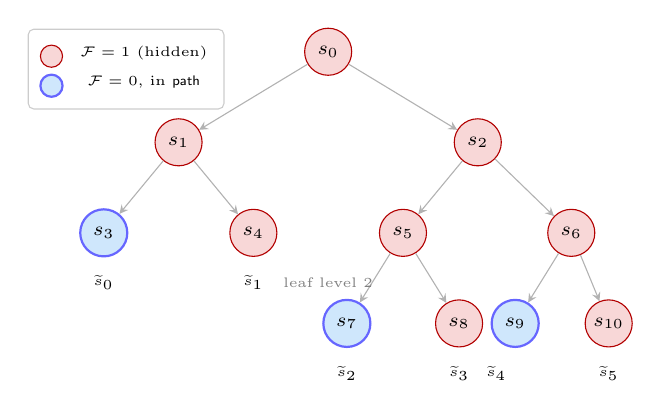
\begin{tikzpicture}[x=0.95cm, y=1.15cm]
  % ---- nodes (final state after all 3 phases) ----
  % Level 0
  \node[hidnode]  (s0)  at (3.5, 0)   {$s_0$};
  % Level 1
  \node[hidnode]  (s1)  at (1.5,-1)   {$s_1$};
  \node[hidnode]  (s2)  at (5.5,-1)   {$s_2$};
  % Level 2  (s3,s4 are leaves; s5,s6 are internal)
  \node[pathnode] (s3)  at (0.5,-2)   {$s_3$};
  \node[hidnode]  (s4)  at (2.5,-2)   {$s_4$};
  \node[hidnode]  (s5)  at (4.5,-2)   {$s_5$};
  \node[hidnode]  (s6)  at (6.75,-2)   {$s_6$};
  % Level 3  (leaves)
  \node[pathnode] (s7)  at (3.75,-3)  {$s_7$};
  \node[hidnode]  (s8)  at (5.25,-3)  {$s_8$};
  \node[pathnode] (s9)  at (6.00,-3)  {$s_9$};
  \node[hidnode]  (s10) at (7.25,-3)  {$s_{10}$};
  % ---- ephemeral-seed labels below leaves ----
  \node[leaflbl] at (0.5,-2.55)  {$\eseed_0$};
  \node[leaflbl] at (2.5,-2.55)  {$\eseed_1$};
  \node[leaflbl] at (3.75,-3.55) {$\eseed_2$};
  \node[leaflbl] at (5.25,-3.55) {$\eseed_3$};
  \node[leaflbl] at (5.75,-3.55) {$\eseed_4$};
  \node[leaflbl] at (7.25,-3.55) {$\eseed_5$};
  % ---- edges ----
  \draw[treeedge] (s0)--(s1); \draw[treeedge] (s0)--(s2);
  \draw[treeedge] (s1)--(s3); \draw[treeedge] (s1)--(s4);
  \draw[treeedge] (s2)--(s5); \draw[treeedge] (s2)--(s6);
  \draw[treeedge] (s5)--(s7); \draw[treeedge] (s5)--(s8);
  \draw[treeedge] (s6)--(s9); \draw[treeedge] (s6)--(s10);
  % ---- "incomplete" annotation ----
  \node[font=\tiny,gray] at (3.5,-2.55) {leaf level~2};
  % ---- legend ----
  \matrix[draw=gray!40, rounded corners=2pt, inner sep=4pt,
          above left=0.2cm and -0.8cm of s1,
          matrix of nodes, nodes={font=\tiny, inner sep=2pt},
          column sep=4pt, row sep=1pt] {
    \node[hidnode,  minimum size=8pt]{}; & \node{$\calF=1$ (hidden)};  \\
    \node[pathnode, minimum size=8pt]{}; & \node{$\calF=0$, in $\tpath$}; \\
  };
\end{tikzpicture}
\caption{LESS-v2 incomplete \GGM\ flag tree, $t=6$, after all three construction
         phases.  Challenge $\mathbf{b}=(0,1,0,1,0,1)$ hides rounds
         $\calH=\{1,3,5\}$.  Path nodes (blue, thick border) give the verifier
         $\eseed_0$, $\eseed_2$, $\eseed_4$.  Injecting a fault on any red node
         exposes the corresponding hidden seed alongside its response, yielding a
         dual revelation.}
\label{fig:less-tree}
\end{figure}


Table~\ref{tab:less-params} lists the parameter sets of LESS.

\begin{table}[tb]
\centering
\caption{LESS-v2 parameter sets~\cite{LESS-spec}.}
\label{tab:less-params}
\begin{tabular}{@{}lcccccc@{}}
\toprule
Parameter set   & $n$ & $k$ & $q$ & $t$ & $w$ & $s$ \\
\midrule
LESS-252-45     & 252 & 126 & 127 &  45 & 34 & 8 \\
LESS-252-68     & 252 & 126 & 127 &  68 & 42 & 4 \\
LESS-252-192    & 252 & 126 & 127 & 192 & 36 & 2 \\
LESS-400-102    & 400 & 200 & 127 & 102 & 61 & 4 \\
LESS-400-220    & 400 & 200 & 127 & 220 & 68 & 2 \\
LESS-548-137    & 548 & 274 & 127 & 137 & 79 & 4 \\
LESS-548-345    & 548 & 274 & 127 & 345 & 75 & 2 \\
\bottomrule
\end{tabular}
\end{table}

% ============================================================
\subsection{MEDS}
\label{sec:meds}
% ============================================================

\paragraph{Context.}
MEDS (Matrix Equivalence Digital Signature)~\cite{ChouNPRRST23} is a code-based
signature scheme whose security rests on the Matrix Code Equivalence Problem
(MCEP).  Like LESS, it applies the Fiat--Shamir transform to a 3-pass Sigma
protocol between a prover holding a secret equivalence
$(A, B) \in \GL_k(q) \times \GL_n(q)$ and a verifier.

\paragraph{Tree type.}
MEDS uses a \emph{complete} binary \GGM\ seed tree to generate $t$ ephemeral
seeds.  Each leaf seed $\eseed_i$ expands into an ephemeral matrix pair.  The
binary challenge vector $\mathbf{h} = (h_0, \ldots, h_{t-1}) \in \{0,1\}^t$
determines which seeds are revealed ($h_i = 0$) and which are hidden ($h_i = 1$).

\paragraph{Reference tree.}
MEDS uses a \emph{Reference Tree} (also called $\SeedTree$) with a
$\SeedTreePaths$ algorithm.  This traverses the tree bottom-up and returns the
minimal set of internal nodes sufficient to reconstruct all revealed leaf seeds,
while no hidden seed $\eseed_i$ (with $h_i = 1$) is derivable.  The three
abstract phases map as follows:
\begin{enumerate}
  \item \textbf{Expansion.}
        $\BuildSeeds(\seed_r, \salt)$ expands from the root to all $t$ leaves via
        $\PRG(\text{node} \,\|\, \salt \,\|\, \text{index}) \to (\text{left},\,\text{right})$.
  \item \textbf{Selection.}
        $\SeedTreePaths(\calT, \mathbf{h})$ marks and collects the publishing nodes.
  \item \textbf{Reconstruction (verifier).}
        $\ReconstructSeeds(\tpath, \mathbf{h}, \salt)$ re-expands only from the
        published nodes.
\end{enumerate}

\paragraph{Secret-extraction opportunity.}
For round $i$ with $h_i = 1$, the signer reveals its ZK response.  If an attacker
obtains both the response and $\eseed_i$, the secret equivalence pair $(A, B)$ is
recoverable by linear algebra.  The Reference Tree is the sole enforcement mechanism
preventing this dual revelation.

\begin{example}
Figure~\ref{fig:meds-tree} shows a complete \GGM\ tree for $t = 4$ with
challenge $\mathbf{h} = (0,1,0,1)$, so $\calH = \{1,3\}$ and $\calR = \{0,2\}$.
Nodes $s_3$ and $s_5$ enter $\tpath$.
\end{example}

\begin{figure}[tb]
\centering
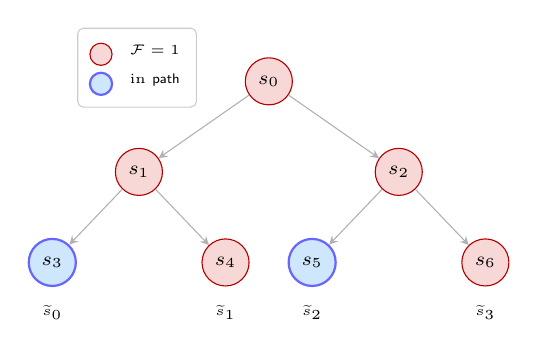
\begin{tikzpicture}[x=1.1cm, y=1.15cm]
  % Level 0
  \node[hidnode]  (s0) at (2,  0)  {$s_0$};
  % Level 1
  \node[hidnode]  (s1) at (0.5,-1) {$s_1$};
  \node[hidnode]  (s2) at (3.5,-1) {$s_2$};
  % Level 2 (leaves)
  \node[pathnode] (s3) at (-0.5,-2){$s_3$};
  \node[hidnode]  (s4) at ( 1.5,-2){$s_4$};
  \node[pathnode] (s5) at ( 2.5,-2){$s_5$};
  \node[hidnode]  (s6) at ( 4.5,-2){$s_6$};
  % Ephemeral seed labels
  \node[leaflbl] at (-0.5,-2.55){$\eseed_0$};
  \node[leaflbl] at ( 1.5,-2.55){$\eseed_1$};
  \node[leaflbl] at ( 2.5,-2.55){$\eseed_2$};
  \node[leaflbl] at ( 4.5,-2.55){$\eseed_3$};
  % Edges
  \draw[treeedge] (s0)--(s1); \draw[treeedge] (s0)--(s2);
  \draw[treeedge] (s1)--(s3); \draw[treeedge] (s1)--(s4);
  \draw[treeedge] (s2)--(s5); \draw[treeedge] (s2)--(s6);
  % Legend
  \matrix[draw=gray!40, rounded corners=2pt, inner sep=4pt,
          above right=0.6cm and -1cm of s1,
          matrix of nodes, nodes={font=\tiny, inner sep=2pt},
          column sep=4pt, row sep=1pt] {
    \node[hidnode,  minimum size=8pt]{}; & \node{$\calF=1$};  \\
    \node[pathnode, minimum size=8pt]{}; & \node{in $\tpath$}; \\
  };
\end{tikzpicture}
\caption{MEDS complete \GGM\ flag tree, $t=4$.
         Challenge $\mathbf{h}=(0,1,0,1)$ hides $\calH=\{1,3\}$.
         Path nodes $s_3$ and $s_5$ (blue) give the verifier $\eseed_0$ and
         $\eseed_2$.  A fault on $s_4$ or $s_6$ exposes the corresponding hidden
         seed alongside its ZK response.}
\label{fig:meds-tree}
\end{figure}

\begin{table}[tb]
\centering
\caption{MEDS parameter sets~\cite{ChouNPRRST23}.}
\label{tab:meds-params}
\begin{tabular}{@{}lccccc@{}}
\toprule
Parameter set & $n$ & $k$ & $q$ & $t$ & $s$ \\
\midrule
MEDS-9923b    & 14 &  7 & 509 & 192 & 2 \\
MEDS-13220b   & 22 & 11 & 127 & 192 & 2 \\
MEDS-41711b   & 30 & 15 & 509 & 392 & 2 \\
\bottomrule
\end{tabular}
\end{table}

% ============================================================
\subsection{CROSS}
\label{sec:cross}
% ============================================================

\paragraph{Context.}
CROSS (Codes and Restricted Objects Signature Scheme)~\cite{CROSSspec} is based on
the Restricted Syndrome Decoding Problem (R-SDP)~\cite{BaldiBPSWW24} and applies the
Fiat--Shamir transform to a 5-pass ($q_2$-identification) protocol.
Like MEDS, CROSS uses a \emph{binary} fixed-weight challenge vector
$\mathbf{c} = (c_0, \ldots, c_{t-1}) \in \{0,1\}^t$ of weight $w$,
so the hidden and revealed index sets are
$\calH = \{i : c_i = 1\}$ and $\calR = \{i : c_i = 0\}$,
identical in structure to MEDS.

\paragraph{Tree type.}
CROSS uses a complete \GGM\ seed tree.  Round~1 of CROSS uses the same
complete binary tree as LESS-v1.  The Round~2 specification~\cite{CROSSspec}
adopts a combined seed-and-Merkle-tree structure, but the seed-publishing
component remains structurally equivalent to the $\SeedTreePaths$ mechanism
of MEDS (Section~\ref{sec:meds}).

\paragraph{Publishing mechanism.}
Flag propagation follows exactly the same three-phase bottom-up rule as
MEDS: initialise all flags to~$0$ except the root, label leaves from the
binary challenge, propagate upward by disjunction.  The published path gives
the verifier access to all $\eseed_i$ with $c_i = 0$, while every $\eseed_i$
with $c_i = 1$ remains hidden.  The structural identity with MEDS means
that every fault location identified for MEDS (Section~\ref{sec:meds}) applies
to CROSS without modification.

\paragraph{Secret-extraction opportunity.}
For round $i$ with $c_i = 1$, the signer reveals a ZK response encoding the
relationship between $\eseed_i$ and the long-term secret R-SDP solution.
If an attacker obtains both the response and $\eseed_i$, the secret is
recoverable by the linear-algebra argument of ZKFault~\cite{ZKFault},
which demonstrated full key recovery from a single fault for all CROSS
parameter sets.

\begin{example}
Figure~\ref{fig:cross-tree} shows a complete \GGM\ tree for $t = 4$ with
binary challenge $\mathbf{c} = (0,1,0,1)$, so $\calH = \{1,3\}$ and
$\calR = \{0,2\}$.  Nodes $s_3$ and $s_5$ enter $\tpath$.
The tree topology and the flag-propagation logic are identical to the MEDS
example of Figure~\ref{fig:meds-tree}; only the underlying hard problem
and response format differ.  A fault on $s_4$ or $s_6$ exposes the
corresponding hidden seed alongside its R-SDP response, enabling recovery
of the long-term secret.
\end{example}

\begin{figure}[tb]
\centering
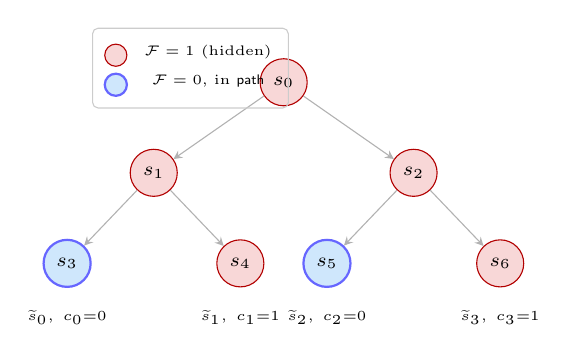
\begin{tikzpicture}[x=1.1cm, y=1.15cm]
  % Level 0
  \node[hidnode]  (s0) at (2,  0)  {$s_0$};
  % Level 1
  \node[hidnode]  (s1) at (0.5,-1) {$s_1$};
  \node[hidnode]  (s2) at (3.5,-1) {$s_2$};
  % Level 2 (leaves)
  \node[pathnode] (s3) at (-0.5,-2){$s_3$};
  \node[hidnode]  (s4) at ( 1.5,-2){$s_4$};
  \node[pathnode] (s5) at ( 2.5,-2){$s_5$};
  \node[hidnode]  (s6) at ( 4.5,-2){$s_6$};
  % Ephemeral-seed labels + challenge values
  \node[leaflbl] at (-0.5,-2.6){$\eseed_0,\; c_0{=}0$};
  \node[leaflbl] at ( 1.5,-2.6){$\eseed_1,\; c_1{=}1$};
  \node[leaflbl] at ( 2.5,-2.6){$\eseed_2,\; c_2{=}0$};
  \node[leaflbl] at ( 4.5,-2.6){$\eseed_3,\; c_3{=}1$};
  % Edges
  \draw[treeedge] (s0)--(s1); \draw[treeedge] (s0)--(s2);
  \draw[treeedge] (s1)--(s3); \draw[treeedge] (s1)--(s4);
  \draw[treeedge] (s2)--(s5); \draw[treeedge] (s2)--(s6);
  % Legend
  \matrix[draw=gray!40, rounded corners=2pt, inner sep=4pt,
          above right=0.6cm and -1cm of s1,
          matrix of nodes, nodes={font=\tiny, inner sep=2pt},
          column sep=4pt, row sep=1pt] {
    \node[hidnode,  minimum size=8pt]{}; & \node{$\calF=1$ (hidden)};  \\
    \node[pathnode, minimum size=8pt]{}; & \node{$\calF=0$, in $\tpath$}; \\
  };
\end{tikzpicture}
\caption{CROSS complete \GGM\ flag tree, $t=4$, binary challenge
         $\mathbf{c}=(0,1,0,1)$.  The tree structure is identical to the MEDS
         example (Figure~\ref{fig:meds-tree}): path nodes $s_3$ and $s_5$ (blue)
         give the verifier $\eseed_0$ and $\eseed_2$.  A fault on $s_4$ or
         $s_6$ exposes the corresponding hidden seed alongside its R-SDP
         response, enabling full key recovery as shown in ZKFault~\cite{ZKFault}.}
\label{fig:cross-tree}
\end{figure}

% ============================================================
\subsection{MPCitH / VOLEitH Family (FAEST, Mirath, SDitH, RYDE)}
\label{sec:mpcith}
% ============================================================

\paragraph{Context.}
MPC-in-the-Head (MPCitH) schemes use the \GGM tree in a more
elaborate but structurally analogous way.  They generate $N$ virtual
\emph{party shares} for each of $\tau$ parallel repetitions.  For repetition $e$,
the Fiat--Shamir challenge selects one hidden party index
$i^*_e \in \{0, \ldots, N-1\}$.  The \GGM\ tree lets the signer reveal all $N-1$
non-hidden shares using $O(\log N)$ published intermediate seeds.

\paragraph{Tree types.}
\begin{itemize}
  \item \textbf{Classic MPCitH (Mirath, RYDE).}
        A forest of $\tau$ independent complete binary trees, each with $N$
        leaves.  All roots are derived from a single master seed via $\XOF$.
  \item \textbf{VOLEitH (FAEST, SDitH v2).}
        A single large \GGM\ tree with $\tau \times N$ leaves, as described
        in~\cite{OneTree}.  Child-node generation uses $\PRG = \text{AES-CTR}$
        (FAEST) or SHAKE (SDitH).
\end{itemize}

The all-but-one vector commitment (AVC / BAVC) mechanism is the MPCitH counterpart
of the flag tree.  For each repetition $e$, the signer publishes the
\emph{co-path}: the sequence of sibling nodes along the path from the hidden leaf
$i^*_e$ to the root.  The verifier can re-expand all $N-1$ non-hidden leaf seeds
from the co-path alone.  This is structurally the \GGM-path mechanism with
exactly one hidden leaf per repetition, and the same fault surfaces (index
arithmetic, loop increments, conditional branch) apply.

In LESS, MEDS, and CROSS, the secret is a permutation or matrix equivalence
embedded in the hidden seed's ephemeral commitment.  In MPCitH, the hidden seed
generates the prover's witness share.  In both cases the invariant is identical:
the signer must never simultaneously reveal both the hidden leaf seed \emph{and}
the corresponding ZK response for the same round.


\section{Abstract Model}
\label{sec:abstract}

We now define a scheme-agnostic abstraction that captures the common structure
of the \GGM-tree mechanism across all schemes discussed in
Section~\ref{sec:background}.

\begin{definition}[\GZKST]
\sloppy
\label{def:gzkst}
A \emph{Generic ZK Seed Tree} (\GZKST) is a tuple
$\Pi = (\Setup,\, \Expand,\, \Chal,\, \Decide,\, \Publish,\, \Recon)$
parametrised by:
\begin{itemize}
  \item $\lam$: the security parameter;
  \item $t \in \mathbb{N}$: the number of parallel ZK repetitions;
  \item $\PRG : \{0,1\}^{\lam} \to \{0,1\}^{2\lam}$: a secure pseudorandom generator;
  \item $\calS$: the \emph{secret type}
        (e.g., permutations for LESS, matrix pairs for MEDS, party shares for MPCitH).
\end{itemize}
The six algorithms are:
\begin{enumerate}
  \item $\Setup(1^{\lam}) \to (\seed_r, \salt)$:
        samples a master seed $\seed_r \getsr \{0,1\}^{\lam}$ and a public salt.
  \item $\Expand(\seed_r, \salt) \to (\calT, (\eseed_0, \ldots, \eseed_{t-1}))$:
        builds a binary tree $\calT$ by top-down \PRG-expansion from $\seed_r$.
        Each leaf $i \in \{0, \ldots, t-1\}$ holds a seed $\eseed_i$.
        Tree topology may be complete or incomplete (scheme-dependent).
  \item $\Chal(\cmt, \msg) \to \mathbf{c} = (c_0, \ldots, c_{t-1})$:
        derives a Fiat--Shamir challenge from the commitment and message.
        $c_i = 0$ indicates that round $i$ requires the ephemeral seed;
        $c_i \neq 0$ indicates a secret-dependent response.
  \item $\Decide(\mathbf{c}) \to (\calH, \calR)$:
        partitions $\{0, \ldots, t-1\}$ into the hidden index set
        $\calH = \{i : c_i \neq 0\}$ and the revealed index set
        $\calR = \{i : c_i = 0\}$.
  \item $\Publish(\calT, \calH) \to \tpath$:
        constructs a flag structure $\calF : V(\calT) \to \{0,1\}$ and returns the
        minimal set of nodes $\tpath$ from which every $\eseed_i$ with
        $i \in \calR$ is reconstructible, while no $\eseed_i$ with
        $i \in \calH$ is derivable.
  \item $\Recon(\tpath, \mathbf{c}, \salt) \to \{\eseed_i : i \in \calR\}$:
        verifier-side reconstruction of revealed leaf seeds from $\tpath$.
\end{enumerate}
\end{definition}

% ------------------------------------------------------------
\subsection{The Flag Structure}
\label{sec:flag-structure}
% ------------------------------------------------------------

The flag structure $\calF$ produced internally by $\Publish$ is the key
intermediate object.  It is a labelling $\calF : V(\calT) \to \{0,1\}$ where:
\begin{itemize}
  \item $\calF(v) = 0$: node $v$ is \emph{publishable}---either
        directly included in $\tpath$ or derivable from a published ancestor;
  \item $\calF(v) = 1$: node $v$ is \emph{hidden}---it must not appear in
        $\tpath$ and must not be derivable from published nodes.
\end{itemize}

\noindent
The flag structure satisfies two invariants:

\begin{invariant}[Correctness]
\label{inv:correctness}
For every $i \in \calR$ there exists a node $v$ on the path from the root to
leaf $\eseed_i$ such that $\calF(v) = 0$ and $\calF(\mathsf{parent}(v)) = 1$.
\end{invariant}

\begin{invariant}[ZK hiding]
\label{inv:hiding}
For every $i \in \calH$, no ancestor of leaf $\eseed_i$ satisfies $\calF(v) = 0$.
\end{invariant}

The ZK property of the signature scheme is contingent on
Invariant~\ref{inv:hiding} holding for \emph{all} $i \in \calH$.  A fault that
changes $\calF(v)$ from $1$ to $0$ for any $v$ that is an ancestor of some
$\eseed_i$ with $i \in \calH$ \emph{breaks Invariant~\ref{inv:hiding}} and
may allow an attacker to reconstruct $\eseed_i$.

% ------------------------------------------------------------
\subsection{Mapping Schemes to the GZKST Model}
\label{sec:mapping}

We propose in this section to segment each of the ZK-based PQ signatures aforementionned into the elements of the GZKST tuple we defined in \ref{def:gzkst}.





% ------------------------------------------------------------



\subsubsection{LESS-V2}

\begin{itemize}
    \item $\Setup(1^{\lam}) \to (\seed_r, \salt)$ The root seed is sampled using the secret key seed. The salt is sampled uniformly at random.
    \item $\Expand(\seed_r, \salt) \to (\calT, (\eseed_0, \ldots, \eseed_{t-1}))$ 
LESS-v2 uses an \emph{incomplete} \GGM\ tree with $T = \lceil \log_2 t \rceil$
levels.  Leaves are distributed across the bottom two levels; the index offsets
are tracked via the arrays $\mathsf{npl}$, $\mathsf{ll}$, $\mathsf{off}$, and
$\mathsf{lsi}$.

    \item $\Chal(\cmt, \msg) \to \mathbf{c} = (c_0, \ldots, c_{t-1})$ In LESS, the commitment fed into the Fiat--Shamir hash is the concatenation
of all $t$ canonical-form matrices $\mathbf{B}^{(1)}, \ldots, \mathbf{B}^{(t)}$
together with the salt and the message.
The resulting digest \textsf{cmt} is then passed to \textsf{SampleChallenge}, which produces the challenge vector
$\mathbf{b} = (b^{(1)}, \ldots, b^{(t)}) \in \{0, \ldots, s-1\}^t$
of fixed weight $w$, where each non-zero entry $b^{(i)} \in \{1, \ldots, s-1\}$
indexes one of the $s-1$ public keys.
In the framework notation, the challenge value per round is
$c_i = b^{(i)}$: the condition $c_i = 0$ signals that round $i$ requires the
ephemeral seed $\eseed^{(i)}$, while $c_i \neq 0$ signals that a
secret-dependent coset representative must be provided instead.

    \item $\Decide(\mathbf{c}) \to (\calH, \calR)$ From the challenge vector $\mathbf{b}$, LESS computes the support
$U = \mathrm{supp}(\mathbf{b})$, i.e., the set of indices $i$ for
which $b^{(i)} \neq 0$. This directly induces the partition required by the framework.
    \item $\Publish(\calT, \calH) \to \tpath$  
    \paragraph{Flag tree.} LESS-v2 constructs an auxiliary
\emph{flag tree} of the same shape as the seed tree.  It is a labelling
$\calF : V(\calT) \to \{0,1\}$ where $\calF(v) = 0$ marks a publishable
node and $\calF(v) = 1$ marks a hidden node.  The flag tree is built in three
sequential phases:
\begin{enumerate}
  \item \textbf{Initialisation.}  Every node is set to $0$ except the root,
        which is set to $1$.
  \item \textbf{Leaf labelling} ($\LabelLeaves$).  For each leaf $i$, set
        \begin{equation*}
          \calF(\mathrm{leaf}_i) =
          \begin{cases} 1 & \text{if } b[i] \neq 0, \\ 0 & \text{otherwise,} \end{cases}
        \end{equation*}
        where $\mathbf{b} = (b[0], \ldots, b[t-1])$ is the Fiat--Shamir challenge
        vector of weight $w$ over the alphabet $\{0, \ldots, s-1\}$.
  \item \textbf{Upward propagation} ($\ComputeSeeds$).  For each internal node $v$
        with children $\ell$ and $r$:
        \begin{equation*}
          \calF(v) = \calF(\ell) \vee \calF(r).
        \end{equation*}
        This ensures the minimum set of nodes is published to reconstruct all
        revealed leaf seeds.
\end{enumerate}
The path is then constructed from the top down following this logic : if a node is flagged as true and its parent node is flagged as false, the seed in the current node is added to the path.

\item $\Recon(\tpath, \mathbf{c}, \salt) \to \{\eseed_i : i \in \calR\}$ 

On the verifier side, $\mathsf{PathToSeedTree}_t(h_0, \ldots, h_{t-1},\,
p,\, \alpha)$ reconstructs an empty tree of the same shape, places the
received path nodes at their correct positions, and re-expands each
downward via the PRG $\mathrm{G}$ until all $t$ leaf positions are
filled.
Positions $i \in \mathcal{H}$ are left empty (no seed on their
root-to-leaf path was ever published), while positions $i \in \mathcal{R}$
yield the recovered seeds $\sigma_i$, from which the verifier
re-derives $(\tilde{\mathbf{A}}_i, \tilde{\mathbf{B}}_i)$ and
re-computes $\tilde{\mathbf{G}}_i$ to verify the commitment $d$.

\end{itemize}




\begin{example}
Figure~\ref{fig:less-tree} illustrates an incomplete \GGM\ tree for $t = 6$ with
challenge $\mathbf{b} = (0,1,0,1,0,1)$, so
$\calH = \{1,3,5\}$ and $\calR = \{0,2,4\}$.
After all three phases, nodes $s_3$, $s_7$, and $s_9$ satisfy
$\calF(v)=0$ with $\calF(\mathsf{parent}(v))=1$ and thus enter $\tpath$,
giving the verifier access to $\eseed_0$, $\eseed_2$, and $\eseed_4$.
\end{example}

\begin{figure}[tb]
\centering
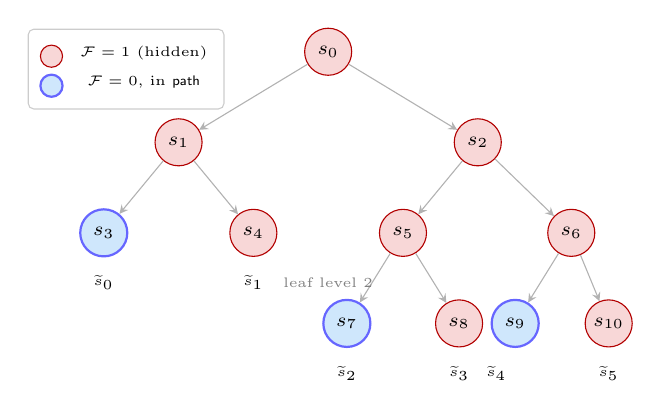
\begin{tikzpicture}[x=0.95cm, y=1.15cm]
  % ---- nodes (final state after all 3 phases) ----
  % Level 0
  \node[hidnode]  (s0)  at (3.5, 0)   {$s_0$};
  % Level 1
  \node[hidnode]  (s1)  at (1.5,-1)   {$s_1$};
  \node[hidnode]  (s2)  at (5.5,-1)   {$s_2$};
  % Level 2  (s3,s4 are leaves; s5,s6 are internal)
  \node[pathnode] (s3)  at (0.5,-2)   {$s_3$};
  \node[hidnode]  (s4)  at (2.5,-2)   {$s_4$};
  \node[hidnode]  (s5)  at (4.5,-2)   {$s_5$};
  \node[hidnode]  (s6)  at (6.75,-2)   {$s_6$};
  % Level 3  (leaves)
  \node[pathnode] (s7)  at (3.75,-3)  {$s_7$};
  \node[hidnode]  (s8)  at (5.25,-3)  {$s_8$};
  \node[pathnode] (s9)  at (6.00,-3)  {$s_9$};
  \node[hidnode]  (s10) at (7.25,-3)  {$s_{10}$};
  % ---- ephemeral-seed labels below leaves ----
  \node[leaflbl] at (0.5,-2.55)  {$\eseed_0$};
  \node[leaflbl] at (2.5,-2.55)  {$\eseed_1$};
  \node[leaflbl] at (3.75,-3.55) {$\eseed_2$};
  \node[leaflbl] at (5.25,-3.55) {$\eseed_3$};
  \node[leaflbl] at (5.75,-3.55) {$\eseed_4$};
  \node[leaflbl] at (7.25,-3.55) {$\eseed_5$};
  % ---- edges ----
  \draw[treeedge] (s0)--(s1); \draw[treeedge] (s0)--(s2);
  \draw[treeedge] (s1)--(s3); \draw[treeedge] (s1)--(s4);
  \draw[treeedge] (s2)--(s5); \draw[treeedge] (s2)--(s6);
  \draw[treeedge] (s5)--(s7); \draw[treeedge] (s5)--(s8);
  \draw[treeedge] (s6)--(s9); \draw[treeedge] (s6)--(s10);
  % ---- "incomplete" annotation ----
  \node[font=\tiny,gray] at (3.5,-2.55) {leaf level~2};
  % ---- legend ----
  \matrix[draw=gray!40, rounded corners=2pt, inner sep=4pt,
          above left=0.2cm and -0.8cm of s1,
          matrix of nodes, nodes={font=\tiny, inner sep=2pt},
          column sep=4pt, row sep=1pt] {
    \node[hidnode,  minimum size=8pt]{}; & \node{$\calF=1$ (hidden)};  \\
    \node[pathnode, minimum size=8pt]{}; & \node{$\calF=0$, in $\tpath$}; \\
  };
\end{tikzpicture}
\caption{LESS-v2 incomplete \GGM\ flag tree, $t=6$, after all three construction
         phases.  Challenge $\mathbf{b}=(0,1,0,1,0,1)$ hides rounds
         $\calH=\{1,3,5\}$.  Path nodes (blue, thick border) give the verifier
         $\eseed_0$, $\eseed_2$, $\eseed_4$.  Injecting a fault on any red node
         exposes the corresponding hidden seed alongside its response, yielding a
         dual revelation.}
\label{fig:less-tree}
\end{figure}


Table~\ref{tab:less-params} lists the parameter sets of LESS.

\begin{table}[tb]
\centering
\caption{LESS-v2 parameter sets~\cite{LESS-spec}.}
\label{tab:less-params}
\begin{tabular}{@{}lcccccc@{}}
\toprule
Parameter set   & $n$ & $k$ & $q$ & $t$ & $w$ & $s$ \\
\midrule
LESS-252-45     & 252 & 126 & 127 &  45 & 34 & 8 \\
LESS-252-68     & 252 & 126 & 127 &  68 & 42 & 4 \\
LESS-252-192    & 252 & 126 & 127 & 192 & 36 & 2 \\
LESS-400-102    & 400 & 200 & 127 & 102 & 61 & 4 \\
LESS-400-220    & 400 & 200 & 127 & 220 & 68 & 2 \\
LESS-548-137    & 548 & 274 & 127 & 137 & 79 & 4 \\
LESS-548-345    & 548 & 274 & 127 & 345 & 75 & 2 \\
\bottomrule
\end{tabular}
\end{table}

\subsubsection{MEDS}

\begin{itemize}
    \item $\Setup(1^{\lam}) \to (\seed_r, \salt)$ 
    
    MEDS samples a fresh $\ell_{\mathrm{sec\_seed}}$-byte random scalar, then derives both the master tree seed
$\rho \in \mathcal{B}^{\ell_{\mathrm{tree\_seed}}}$ and the public salt
$\alpha \in \mathcal{B}^{\ell_{\mathrm{salt}}}$ in a single XOF call. 
    \item $\Expand(\seed_r, \salt) \to (\calT, (\eseed_0, \ldots, \eseed_{t-1}))$ 
    
    From $(\rho, \alpha)$, MEDS calls $\mathsf{SeedTree}_t(\rho, \alpha)$
(line~13) to build a complete binary tree of height
$\lceil \log_2 t \rceil$ and return its first $t$ leaves
$\sigma_0, \ldots, \sigma_{t-1} \in \mathcal{B}^{\ell_{\mathrm{tree\_seed}}}$.
    \item $\Chal(\cmt, \msg) \to \mathbf{c} = (c_0, \ldots, c_{t-1})$ 
    
    Each leaf $\sigma_i$ is then expanded into three sub-seeds
$(\sigma_{\tilde{A}_i},\, \sigma_{\tilde{B}_i},\, \sigma_i')$ with $\mathrm{XOF}$.
from which ephemeral invertible matrices sampled then generator matrixes computed.
The commitment is formed by hashing the compressed systematic forms of all
$t$ ephemeral generator matrices $\tilde{\mathbf{G}}_0, \ldots,
\tilde{\mathbf{G}}_{t-1}$ together with the message $m$.

The digest $d$ is then parsed by $\mathsf{ParseHash}_{s,t,w}(d)$
to produce the challenge vector
$h_0, \ldots, h_{t-1} \in \{0, \ldots, s-1\}$
of fixed weight $w$.

In the framework notation, $c_i = h_i$. 

    \item $\Decide(\mathbf{c}) \to (\calH, \calR)$ The condition $c_i = 0$ signals
that round $i$ requires the ephemeral seed $\mathsf{es}_i$, while
$c_i \neq 0$ indicates that a secret-dependent matrix response must be
provided.
    \item $\Publish(\calT, \calH) \to \tpath$  
    
    MEDS calls $\mathsf{SeedTreeToPath}_t(h_0, \ldots, h_{t-1},\, \rho,\,
\alpha)$, which rebuilds the full seed tree, then for each
$i \in \mathcal{H}$ removes the label of leaf $i$ and propagates the
deletion upward, erasing every ancestor whose subtree is entirely hidden.
The function then serialises in depth-first order all remaining non-empty
node labels at the highest possible level, zero-padded to
$\ell_{\mathrm{path}}$ bytes, yielding the seed path $p$.

\item $\Recon(\tpath, \mathbf{c}, \salt) \to \{\eseed_i : i \in \calR\}$ 

On the verifier side, $\mathsf{PathToSeedTree}_t(h_0, \ldots, h_{t-1},\,
p,\, \alpha)$ reconstructs an empty tree of the same shape, places the
received path nodes at their correct positions, and re-expands each
downward via the PRG $\mathrm{G}$ until all $t$ leaf positions are
filled.
Positions $i \in \mathcal{H}$ are left empty (no seed on their
root-to-leaf path was ever published), while positions $i \in \mathcal{R}$
yield the recovered seeds $\sigma_i$, from which the verifier
re-derives $(\tilde{\mathbf{A}}_i, \tilde{\mathbf{B}}_i)$ and
re-computes $\tilde{\mathbf{G}}_i$ to verify the commitment $d$.
\end{itemize}


\begin{example}
Figure~\ref{fig:meds-tree} shows a complete \GGM\ tree for $t = 4$ with
challenge $\mathbf{h} = (0,1,0,1)$, so $\calH = \{1,3\}$ and $\calR = \{0,2\}$.
Nodes $s_3$ and $s_5$ enter $\tpath$.
\end{example}

\begin{figure}[tb]
\centering
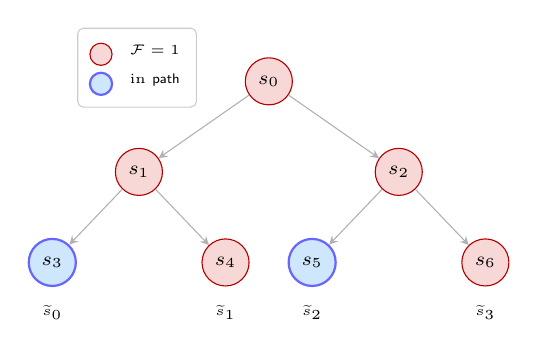
\begin{tikzpicture}[x=1.1cm, y=1.15cm]
  % Level 0
  \node[hidnode]  (s0) at (2,  0)  {$s_0$};
  % Level 1
  \node[hidnode]  (s1) at (0.5,-1) {$s_1$};
  \node[hidnode]  (s2) at (3.5,-1) {$s_2$};
  % Level 2 (leaves)
  \node[pathnode] (s3) at (-0.5,-2){$s_3$};
  \node[hidnode]  (s4) at ( 1.5,-2){$s_4$};
  \node[pathnode] (s5) at ( 2.5,-2){$s_5$};
  \node[hidnode]  (s6) at ( 4.5,-2){$s_6$};
  % Ephemeral seed labels
  \node[leaflbl] at (-0.5,-2.55){$\eseed_0$};
  \node[leaflbl] at ( 1.5,-2.55){$\eseed_1$};
  \node[leaflbl] at ( 2.5,-2.55){$\eseed_2$};
  \node[leaflbl] at ( 4.5,-2.55){$\eseed_3$};
  % Edges
  \draw[treeedge] (s0)--(s1); \draw[treeedge] (s0)--(s2);
  \draw[treeedge] (s1)--(s3); \draw[treeedge] (s1)--(s4);
  \draw[treeedge] (s2)--(s5); \draw[treeedge] (s2)--(s6);
  % Legend
  \matrix[draw=gray!40, rounded corners=2pt, inner sep=4pt,
          above right=0.6cm and -1cm of s1,
          matrix of nodes, nodes={font=\tiny, inner sep=2pt},
          column sep=4pt, row sep=1pt] {
    \node[hidnode,  minimum size=8pt]{}; & \node{$\calF=1$};  \\
    \node[pathnode, minimum size=8pt]{}; & \node{in $\tpath$}; \\
  };
\end{tikzpicture}
\caption{MEDS complete \GGM\ flag tree, $t=4$.
         Challenge $\mathbf{h}=(0,1,0,1)$ hides $\calH=\{1,3\}$.
         Path nodes $s_3$ and $s_5$ (blue) give the verifier $\eseed_0$ and
         $\eseed_2$.  A fault on $s_4$ or $s_6$ exposes the corresponding hidden
         seed alongside its ZK response.}
\label{fig:meds-tree}
\end{figure}

\begin{table}[tb]
\centering
\caption{MEDS parameter sets~\cite{ChouNPRRST23}.}
\label{tab:meds-params}
\begin{tabular}{@{}lccccc@{}}
\toprule
Parameter set & $n$ & $k$ & $q$ & $t$ & $s$ \\
\midrule
MEDS-9923b    & 14 &  7 & 509 & 192 & 2 \\
MEDS-13220b   & 22 & 11 & 127 & 192 & 2 \\
MEDS-41711b   & 30 & 15 & 509 & 392 & 2 \\
\bottomrule
\end{tabular}
\end{table}

\subsubsection{CROSS}

\begin{itemize}
    \item $\Setup(1^{\lam}) \to (\seed_r, \salt)$: The root seed is of size $\lam$ and the salt $2\lam$. They are both theoretically drawn uniformly at random.
    \item $\Expand(\seed_r, \salt) \to (\calT, (\eseed_0, \ldots, \eseed_{t-1}))$: 

CROSS-v1 uses a complete \GGM\ tree identical in structure to LESS-v1.
CROSS-v2 may adopt an optimised variant; the reference implementation uses a
$\SeedTreePaths$ mechanism structurally equivalent to that of MEDS.

The GGM tree in CROSS is a full binary tree where each parent node's $\lam$-bit seed is concatenated with a global salt and the node's unique index, then processed through a CSPRNG (SHAKE) to deterministically produce two $\lam$-bit strings for its left and right children.
      \item $\Chal(\cmt, \msg) \to \mathbf{c} = (c_0, \ldots, c_{t-1})$ 
      
      CROSS applies the Fiat--Shamir transform in two successive rounds.

First, the $t$ commitment pairs $(\mathsf{cmt}_0[i], \mathsf{cmt}_1[i])$,
the salt, and the message are hashed to produce the first challenge vector
$\mathsf{chall}_1 \in (\mathbb{F}_p^*)^t$, from which each first response
$\mathsf{digest}_{y_i} = \mathrm{Hash}({\bf u}'_i + \mathsf{chall}_1[i]
\cdot {\bf e}'_i)$ is derived.

A second hash over all first-challenge digests then yields the
second challenge vector $\mathsf{chall}_2 \in \mathcal{B}(t, w)$ of fixed Hamming weight $w$.
In the framework notation, $c_i = \mathsf{chall}_2[i] \in \{0,1\}$: the
condition $c_i = 0$ signals that round $i$ requires the ephemeral seed
$\mathsf{es}_i$, while $c_i = 1$ signals that a secret-dependent response
$({\bf y}_i, {\bf v}_i)$ must be provided.

  \item $\Decide(\mathbf{c}) \to (\calH, \calR)$

    The challenge vector determines which of the $t$ ephemeral seeds to hide:
$\calH = \{i : c_i \neq 0\}$ and $\calR = \{i : c_i = 0\}$. 

  \item $\Publish(\calT, \calH) \to \tpath$  
  
CROSS computes the seed path $\mathsf{Path}$ by applying the seed-tree
path algorithm to the full tree with respect to $\mathcal{H}$: for each
$i \in \mathcal{H}$, the label of leaf $i$ is removed and all ancestor
labels on its root-to-leaf path are deleted, then the minimal set of
surviving boundary nodes is serialised in depth-first order.
This corresponds to the framework flag structure
$\mathcal{F} : V(\mathcal{T}) \to \{0,1\}$ with $\mathcal{F}(v) = 1$
marking deleted nodes and $\tpath$ being the remaining boundary.

Additionally, CROSS computes a \emph{Merkle proof} $\mathsf{Proof}$ over
the $t$ commitments $\mathsf{cmt}_0[0], \ldots, \mathsf{cmt}_0[t-1]$,
authenticating the $w$ values $\mathsf{cmt}_0[i]$ for $i \in \mathcal{H}$
that the verifier cannot recompute from any revealed seed.

This Merkle proof is a CROSS-specific mechanism with no analogue in LESS
or MEDS, arising from the dual-commitment structure of the underlying
5-pass protocol.
  \item $\Recon(\tpath, \mathbf{c}, \salt) \to \{\eseed_i : i \in \calR\}$ 
  
  On the verifier side, the received $\mathsf{Path}$ nodes are placed onto
an empty tree of the same structure and re-expanded downward via the CSPRNG
until all $t$ leaf positions are populated.
Positions $i \in \mathcal{H}$ remain empty, as no seed on their
root-to-leaf path was ever published; the verifier instead uses the
explicit response $\mathsf{resp}[i] = ({\bf y}_i, {\bf v}_i)$ together
with the Merkle proof to authenticate $\mathsf{cmt}_0[i]$ and verify the
round.

Positions $i \in \mathcal{R}$ yield the recovered seeds $\mathsf{Seed}[i]$,
from which the verifier re-derives $({\bf e}'_i, {\bf u}'_i)$,
recomputes $\mathsf{cmt}_1[i]$, and checks consistency with the signed
commitment digest.

\end{itemize}
\begin{example}
Figure~\ref{fig:cross-tree} shows a complete \GGM\ tree for $t = 4$ with ternary
challenge $\mathbf{c} = (0,\, 2,\, 0,\, 1)$.  Because $c_1 = 2 \neq 0$ and
$c_3 = 1 \neq 0$, the hidden set is $\calH = \{1,3\}$ and the path nodes are
$s_3$ and $s_5$.  Faulting $s_4$ exposes $\eseed_1$ and thereby leaks the
\emph{second} secret component (corresponding to $c_1 = 2$);
faulting $s_6$ leaks the \emph{first} (corresponding to $c_3 = 1$).
\end{example}

\begin{figure}[tb]
\centering
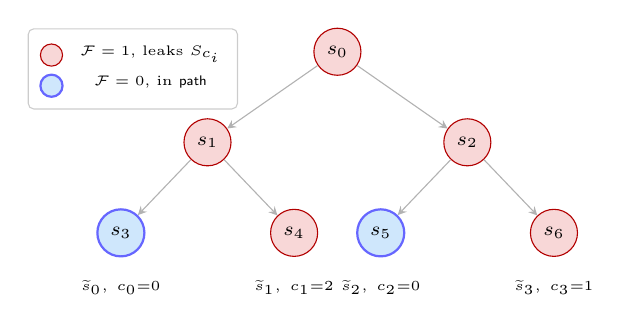
\begin{tikzpicture}[x=1.1cm, y=1.15cm]
  % Level 0
  \node[hidnode]  (s0) at (2,   0) {$s_0$};
  % Level 1
  \node[hidnode]  (s1) at (0.5,-1) {$s_1$};
  \node[hidnode]  (s2) at (3.5,-1) {$s_2$};
  % Level 2 (leaves)
  \node[pathnode] (s3) at (-0.5,-2){$s_3$};
  \node[hidnode]  (s4) at ( 1.5,-2){$s_4$};
  \node[pathnode] (s5) at ( 2.5,-2){$s_5$};
  \node[hidnode]  (s6) at ( 4.5,-2){$s_6$};
  % Ephemeral-seed labels + challenge values
  \node[leaflbl] at (-0.5,-2.6){$\eseed_0,\; c_0{=}0$};
  \node[leaflbl] at ( 1.5,-2.6){$\eseed_1,\; c_1{=}2$};
  \node[leaflbl] at ( 2.5,-2.6){$\eseed_2,\; c_2{=}0$};
  \node[leaflbl] at ( 4.5,-2.6){$\eseed_3,\; c_3{=}1$};
  % Edges
  \draw[treeedge] (s0)--(s1); \draw[treeedge] (s0)--(s2);
  \draw[treeedge] (s1)--(s3); \draw[treeedge] (s1)--(s4);
  \draw[treeedge] (s2)--(s5); \draw[treeedge] (s2)--(s6);
  % Annotations on hidden leaves
  \node[font=\tiny,red!70!black] at (1.5,-2) {\rotatebox{0}{}};
  % Legend
  \matrix[draw=gray!40, rounded corners=2pt, inner sep=4pt,
          above right=0.2cm and -2.5cm of s1,
          matrix of nodes, nodes={font=\tiny, inner sep=2pt},
          column sep=4pt, row sep=1pt] {
    \node[hidnode,  minimum size=8pt]{}; & \node{$\calF=1$, leaks $S_{c_i}$};  \\
    \node[pathnode, minimum size=8pt]{}; & \node{$\calF=0$, in $\tpath$}; \\
  };
\end{tikzpicture}
\caption{CROSS complete \GGM\ flag tree, $t=4$, ternary challenge
         $\mathbf{c}=(0,2,0,1)$.  Faulting hidden node $s_4$ exposes $\eseed_1$
         and leaks the second secret component ($c_1=2$); faulting $s_6$ leaks
         the first ($c_3=1$).  The ternary alphabet means that different hidden
         leaves point to \emph{different} components of the long-term secret.}
\label{fig:cross-tree}
\end{figure}

\subsubsection{MPCitH / VOLEitH Family }

\begin{itemize}
    \item $\Setup(1^{\lam}) \to (\seed_r, \salt)$ TODO
    \item $\Expand(\seed_r, \salt) \to (\calT, (\eseed_0, \ldots, \eseed_{t-1}))$ TODO
    \item $\Chal(\cmt, \msg) \to \mathbf{c} = (c_0, \ldots, c_{t-1})$ TODO
    \item $\Decide(\mathbf{c}) \to (\calH, \calR)$ TODO
    \item $\Publish(\calT, \calH) \to \tpath$  TODO
\end{itemize}


%\section{Fault Model Taxonomy}
%\label{sec:theoretical}
%\subsection{Comparative study of the attack surfaces in state of the art attacks}

\begin{table}[h]
\centering
\caption{Fault Attack mapping of attacks on GZKST-Based Signature Schemes}
\begin{tabular}{@{}lccccc@{}}
\toprule
 & \textbf{LESS} & \textbf{MEDS} & \textbf{CROSS} & \textbf{\begin{tabular}[c]{@{}c@{}}RYDE/\\ Mirath\end{tabular}} & \textbf{FAEST} \\ \midrule
\textbf{\begin{tabular}[c]{@{}l@{}}ZKFault\\ (Mondal et al.)\end{tabular}} & \Publish & \Publish & \begin{tabular}[c]{@{}c@{}} \Publish \\ (not tested)\end{tabular} & - & - \\ \addlinespace
\textbf{\begin{tabular}[c]{@{}l@{}}Fault to Forge\\ (Mondal et al.)\end{tabular}} & \Publish & - & - & - & - \\ \addlinespace
\textbf{\begin{tabular}[c]{@{}l@{}}Faultless Key Recovery\\ (Huang et al.)\end{tabular}} & \Decide & - & - & - & - \\ \addlinespace
\textbf{\begin{tabular}[c]{@{}l@{}}Fault Attack on MPCitH\\ (Banda et al.)\end{tabular}} & - & - & - & \begin{tabular}[c]{@{}c@{}} \Expand, \\ \Chal \end{tabular} & - \\ \addlinespace
\textbf{\begin{tabular}[c]{@{}l@{}}A Case Study on FAEST\\ (Jendral \& Dubrova)\end{tabular}} & - & - & - & - & \Expand \\ \bottomrule
\end{tabular}
\end{table}

\section{Fault Injection attacks on MEDS}
\label{sec:app}
This section details a fault injection (FI) attack against 
the C reference implementation of MEDS. We focus on 
exploiting the tree traversal logic used in the path construction to leak 
hidden seeds.

\paragraph{Target Analysis.}
The primary target of our analysis is the $\SeedTreePath$ function, 
specifically targeting the logic represented in the signing phase of 
the MEDS algorithm (instruction 16 of algorithm~\ref{alg:sign_meds}). 
In the reference implementation\footnote{Reference implementation 
available in \url{https://github.com/MEDSpqc/meds}.}, both $\SeedTreePath$ 
(path generation) and $\SeedTree$ (tree reconstruction) are handled by a unified function, 
\texttt{stree\_to\_path\_to\_stree}, which operates in two modes defined 
by a \texttt{mode} parameter.

\begin{lstlisting}[style=cstyle,caption={minimal description of \texttt{stree\_to\_path\_to\_stree} implementation}., label=lst:path]
void stree_to_path_to_stree(uint8_t *stree, uint8_t *h_digest, uint8_t *path, uint8_t *salt, int mode) {
    ...
    while (1==1) {
        int index_leaf = 0;
        `\highlight{yhl}{while ((indices[id] >> (MEDS\_seed\_tree\_height-h)) == i)}` 
        {// Traverse down toward the secret leaf
            h += 1;
            i <<= 1;
            if (h > MEDS_seed_tree_height) {
                h -= 1;
                i >>= 1;
                `\highlight{rhl}{if (id + 1 < MEDS\_w) id++; }`
                `\highlight{bhl}{index\_leaf = 1;}` // Flag node as hidden
                break;
            }
        }
        ...
    }
}
\end{lstlisting}

The algorithm identifies secret leaves (where $h[i] > 0$) and performs a Depth-First Search (DFS). The exploration halts as soon as it reaches a node that is no longer an ancestor of the hidden leaf. This node is then appended to the signature path. If the exploration reaches a target hidden leaf, the \texttt{index\_leaf} flag is set to ensure the leaf seed remains unpublished and we move on to the next hidden leaf.

\noindent\textbf{Objective.}
The main goal for these attacks is to manipulate the control flow 
via fault injection to leak unpublished seeds (internal nodes or leaves) 
into the public signature path, ultimately compromising the security 
of the signature scheme.

\paragraph{Experimental Setup.}
Our experimental platform consists of a \textbf{CW303-STM32F3} target board, featuring an ARM Cortex-M4 STM32F303RCT7 processor. Clock glitching is performed using a \textbf{ChipWhisperer-Lite}. As a proof-of-concept, the target board is flashed exclusively with the \texttt{stree\_to\_path\_to\_stree} function, using fixed values for the reference tree, salt, and challenge.

%\subsection{Fault Models}
\paragraph{Fault Models.}
We propose three fault models targeting different stages of the tree traversal.

\noindent\textbf{Model 1: Full Tree Recovery (Root Leakage).}
This attack aims to reveal the root seed, which effectively compromises the entire tree. By injecting a fault that causes the skip of the first iteration of \highlight{yhl}{\texttt{while} loop} at line 5 of listing~\ref{lst:path}, the DFS halts immediately at the root ($h=0, i=0$). The root is incorrectly identified as a node ready for publication.

\noindent\textit{Detection and recovery.} The signature path contains only a single non-zero element. Verification is performed by expanding this single seed into a full tree and checking if the resulting signature is accepted.

\noindent\textbf{Model 2: Subtree Recovery.}
By glitching the conditional \highlight{rhl}{\texttt{if (id + 1 < MEDS\_w) id++;}} at line 12 of listing~\ref{lst:path}, the algorithm fails to update the target index \texttt{id}. The traversal logic becomes desynchronized, resulting in the algorithm treating subsequent branches as public. All leaves to the right of the faulted \texttt{id} become computable.
\noindent\textit{Detection and recovery. } This fault is hard to detect without a reference signature. However, one can simulate tree reconstructions for all possible faulted \texttt{id} values to verify which leads to a valid signature. (up to $w$ verifications)

\begin{figure}[H]
\centering
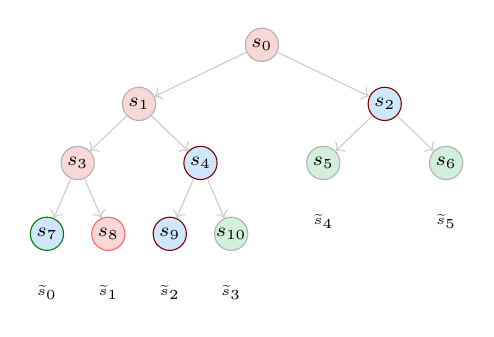
\begin{tikzpicture}[x=0.78cm, y=1.0cm]
  \tikzstyle{neutnode} = [circle, draw=gray!60, fill=nodehid, text=black, minimum size=12pt, inner sep=0pt, font=\scriptsize]
  \tikzstyle{faulted_leaf} = [circle, draw=red!60, fill=nodehid, text=black, minimum size=12pt, inner sep=0pt, font=\scriptsize]
  \tikzstyle{pubnode}  = [circle, draw=green!50!black, fill=nodepath, minimum size=12pt, inner sep=0pt, font=\scriptsize]
  \tikzstyle{fpubnode}  = [circle, draw=red!50!black, fill=nodepath, minimum size=12pt, inner sep=0pt, font=\scriptsize]
  \tikzstyle{zeronode} = [circle, draw=gray!60, fill=nodepub, minimum size=12pt, inner sep=0pt, font=\scriptsize]
  \tikzstyle{treeedge} = [gray!40, rounded corners=2pt,->, thin]
  \tikzstyle{leaflbl}  = [font=\tiny, below=1pt]
  \node[neutnode](s0) at (3.5,0){$s_0$};
  \node[neutnode](s1) at (1.5,-.75){$s_1$};
  \node[fpubnode](s2) at (5.5,-.75){$s_2$};
  \node[neutnode](s3) at (.5,-1.5){$s_3$};
  \node[fpubnode] (s4) at (2.5,-1.5){$s_4$};
  \node[zeronode](s5) at (4.5,-1.5){$s_5$};
  \node[zeronode] (s6) at (6.5,-1.5){$s_6$};
  \node[pubnode] (s7) at (0,-2.4){$s_7$};
  \node[faulted_leaf](s8) at (1,-2.4){$s_8$};
  \node[fpubnode](s9) at (2,-2.4){$s_9$};
  \node[zeronode](s10) at (3,-2.4){$s_{10}$};
  \node[leaflbl] at (0,-2.9){$\eseed_0$};
  \node[leaflbl] at (1,-2.9){$\eseed_1$};
  \node[leaflbl] at (2,-2.9){$\eseed_2$};
  \node[leaflbl] at (3,-2.9){$\eseed_3$};
  \node[leaflbl] at (4.5,-2.0){$\eseed_4$};
  \node[leaflbl] at (6.5,-2.0){$\eseed_5$};
  \draw[treeedge](s0)--(s1);\draw[treeedge](s0)--(s2);
  \draw[treeedge](s1)--(s3);\draw[treeedge](s1)--(s4);
  \draw[treeedge](s2)--(s5);\draw[treeedge](s2)--(s6);
  \draw[treeedge](s3)--(s7);\draw[treeedge](s3)--(s8);
  \draw[treeedge](s4)--(s9);\draw[treeedge](s4)--(s10);
\end{tikzpicture}
\caption{Effect of fault model 2 on the example presented in figure~\ref{fig:less-trees}, if the glitch occured while \texttt{id==1}. The returned path is $\{s_7,s_9,s_4,s_2\}$ and all leaves are computable except $\eseed_1$.}
\label{fig:faulted_path}
\end{figure}

\noindent\textbf{Model 3: Hidden Leaf Recovery.}
This model targets the specific instruction \highlight{bhl}{\texttt{index\_leaf = 1;}} at line 13 of listing~\ref{lst:path}. By skipping this assignment, a hidden leaf is no longer marked as private. The execution continues normally, but the secret leaf seed is copied into the \texttt{path} buffer.

\noindent\textit{Detection and recovery.} The path length will be $w+k$ (where $k > 0$ is the number of iterations of the target instruction that were skipped). Detection involves testing subsets of the path to find a valid signature, which may be computationally expensive ($ \binom{w+k}{w} $ verifications).




\subsection{Results and Observations}

We successfully executed the fault models on the Chipwhisperer board. This section detailed the compiler and glitcher configurations that were required to obtain the desired faults.

\noindent\textbf{Step-by-Step attack.}
For each fault model we first define a target output state signifying a
successful injection, then bracket the target assembly instructions with a
\texttt{trigger\_high()}/\texttt{trigger\_low()} pair so the ChipWhisperer
counts the right clock-cycle window; we verify the disassembly to confirm
compiler optimizations did not move or drop the triggers. The \texttt{repeat}
parameter sets the glitch duration in clock cycles, calibrated from the ARM
nominal cycle counts for the target sequence.

We sweep three parameters to map the fault space: \texttt{width}, the glitch
pulse width (XOR of the system clock, $0\%$--$50\%$ of the clock period);
\texttt{offset}, the phase shift relative to the system clock
($-50\%$--$50\%$); and \texttt{ext\_offset}, the number of clock cycles between
the trigger and the glitch.

\textbf{Model 1: Full tree recovery.}
This attack is successful if the returned path contains a 
single node which is the root node.

\textit{Compilation.} This attack is carried out on a 
code compiled with the default \texttt{-Os} optimization.

\textit{Trigger position.} We directly target the 
evaluation of the conditional and the branching 
instruction corresponding to line 5 of Listing~\ref{lst:path}. 
The compiled result is in Listing~\ref{lst:f1asm}. We fault for 3 
clock cycles.

\begin{lstlisting}[style=asmstyle, label=lst:f1asm, caption=Compiled trigger points for fault model 1.]
0800062c <stree_to_path_to_stree_glitch>:
...
    // trigger_high();
 8000710:	f001 fa12 	bl	8001b38 <trigger_high>
    // while ((indices[id] >> (MEDS_seed_tree_height - h)) == i)
 8000714:	ab06      	add	r3, sp, #24
 8000716:	eb03 0488 	add.w	r4, r3, r8, lsl #2
 800071a:	e00d      	b.n	8000738 <stree_to_path_to_stree_glitch+0x66>
    // trigger_low();
 800071c:	f001 fa13 	bl	8001b46 <trigger_low>
...
\end{lstlisting}

\textit{Parameters.} Figure~\ref{fig:fault1_results} shows that the attack has
 a high success rate and lower reset rates for an \texttt{ext\_offset} ranging 
 from $1.5$ to $2.5$, a small \texttt{offset} of $-1$ to $1$ and rather wide 
 glitches (\texttt{width} over $20$).

\begin{figure}[htp]
    \centering
    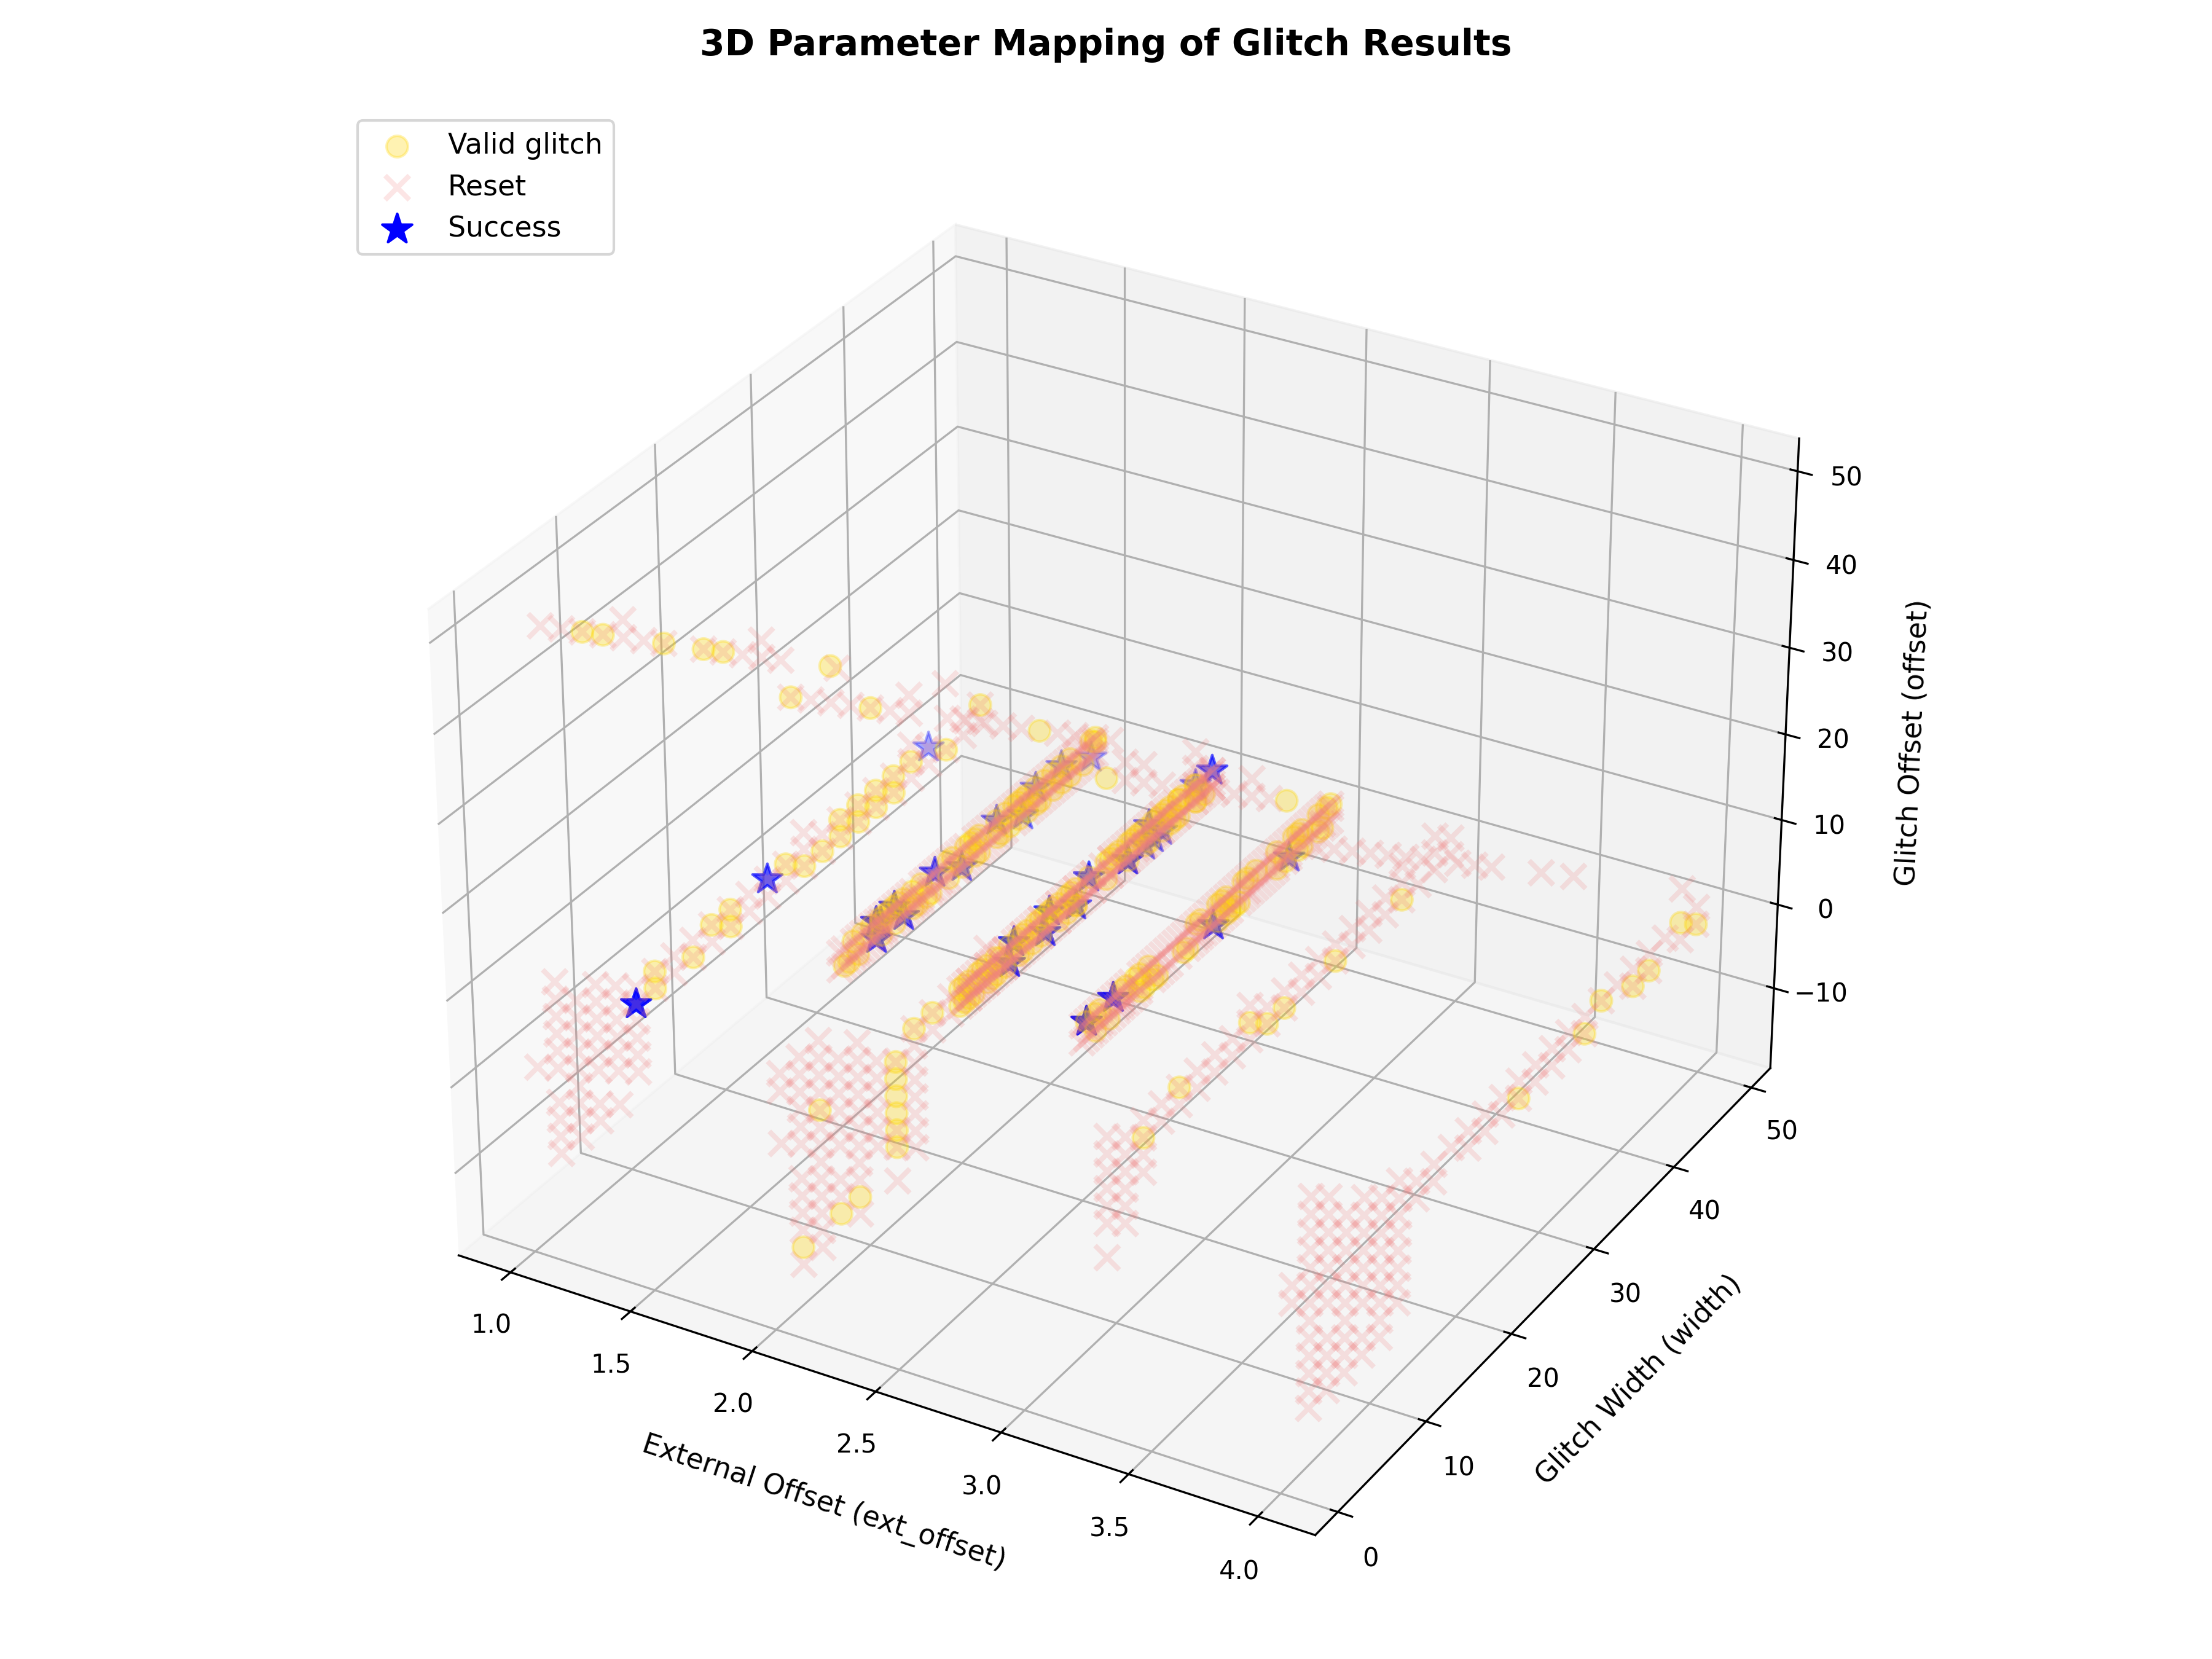
\includegraphics[width=0.62\textwidth]{content/images/glitch_3d_results.png} 
    \caption{Glitch success frequency by glitch width and offset for fault model 1, with 10 tries per parameter set. Valid glitches are runs that did not crash and output paths that were neither correct nor the target faulted path.}
    \label{fig:fault1_results}
\end{figure}

\textbf{Model 2: Subtree recovery.} We consider 
this attack successful if we obtain the faulted path pattern 
described by Figure~\ref{fig:faulted_path}. 

\textit{Compilation.} This is carried out on a code compiled with the default \texttt{-Os} optimization.

\textit{Trigger position.} We set the trigger to frame line $12$ of Listing~\ref{lst:path}. The compiled result is in Listing~\ref{lst:f2asm}.


\begin{lstlisting}[style=asmstyle, label=lst:f2asm, caption=Compiled trigger points for fault model 2.]
080006d2 <stree_to_path_to_stree_glitch>:
...
 8000726:	f001 fa09 	bl	8001b3c <trigger_high> // trigger_high();
 800072a:	f108 0401 	add.w	r4, r8, #1  
 800072e:	2c05      	cmp	r4, #5                 //if (id+1 < MEDS_w)
 8000730:	bf88      	it	hi
 8000732:	4644      	movhi	r4, r8             // id++ ;
 8000734:	f001 fa09 	bl	8001b4a <trigger_low>  // trigger_low();
...
\end{lstlisting}


\textit{Parameters.} The evaluation of the condition and 
the incrementation of \texttt{id} require 3 clock cycles. 
We therefore set \texttt{repeat} to $3$. 
Figure~\ref{fig:fault2_results} shows the success in terms 
of glitch offset and width.

\begin{figure}[htp]
    \centering
    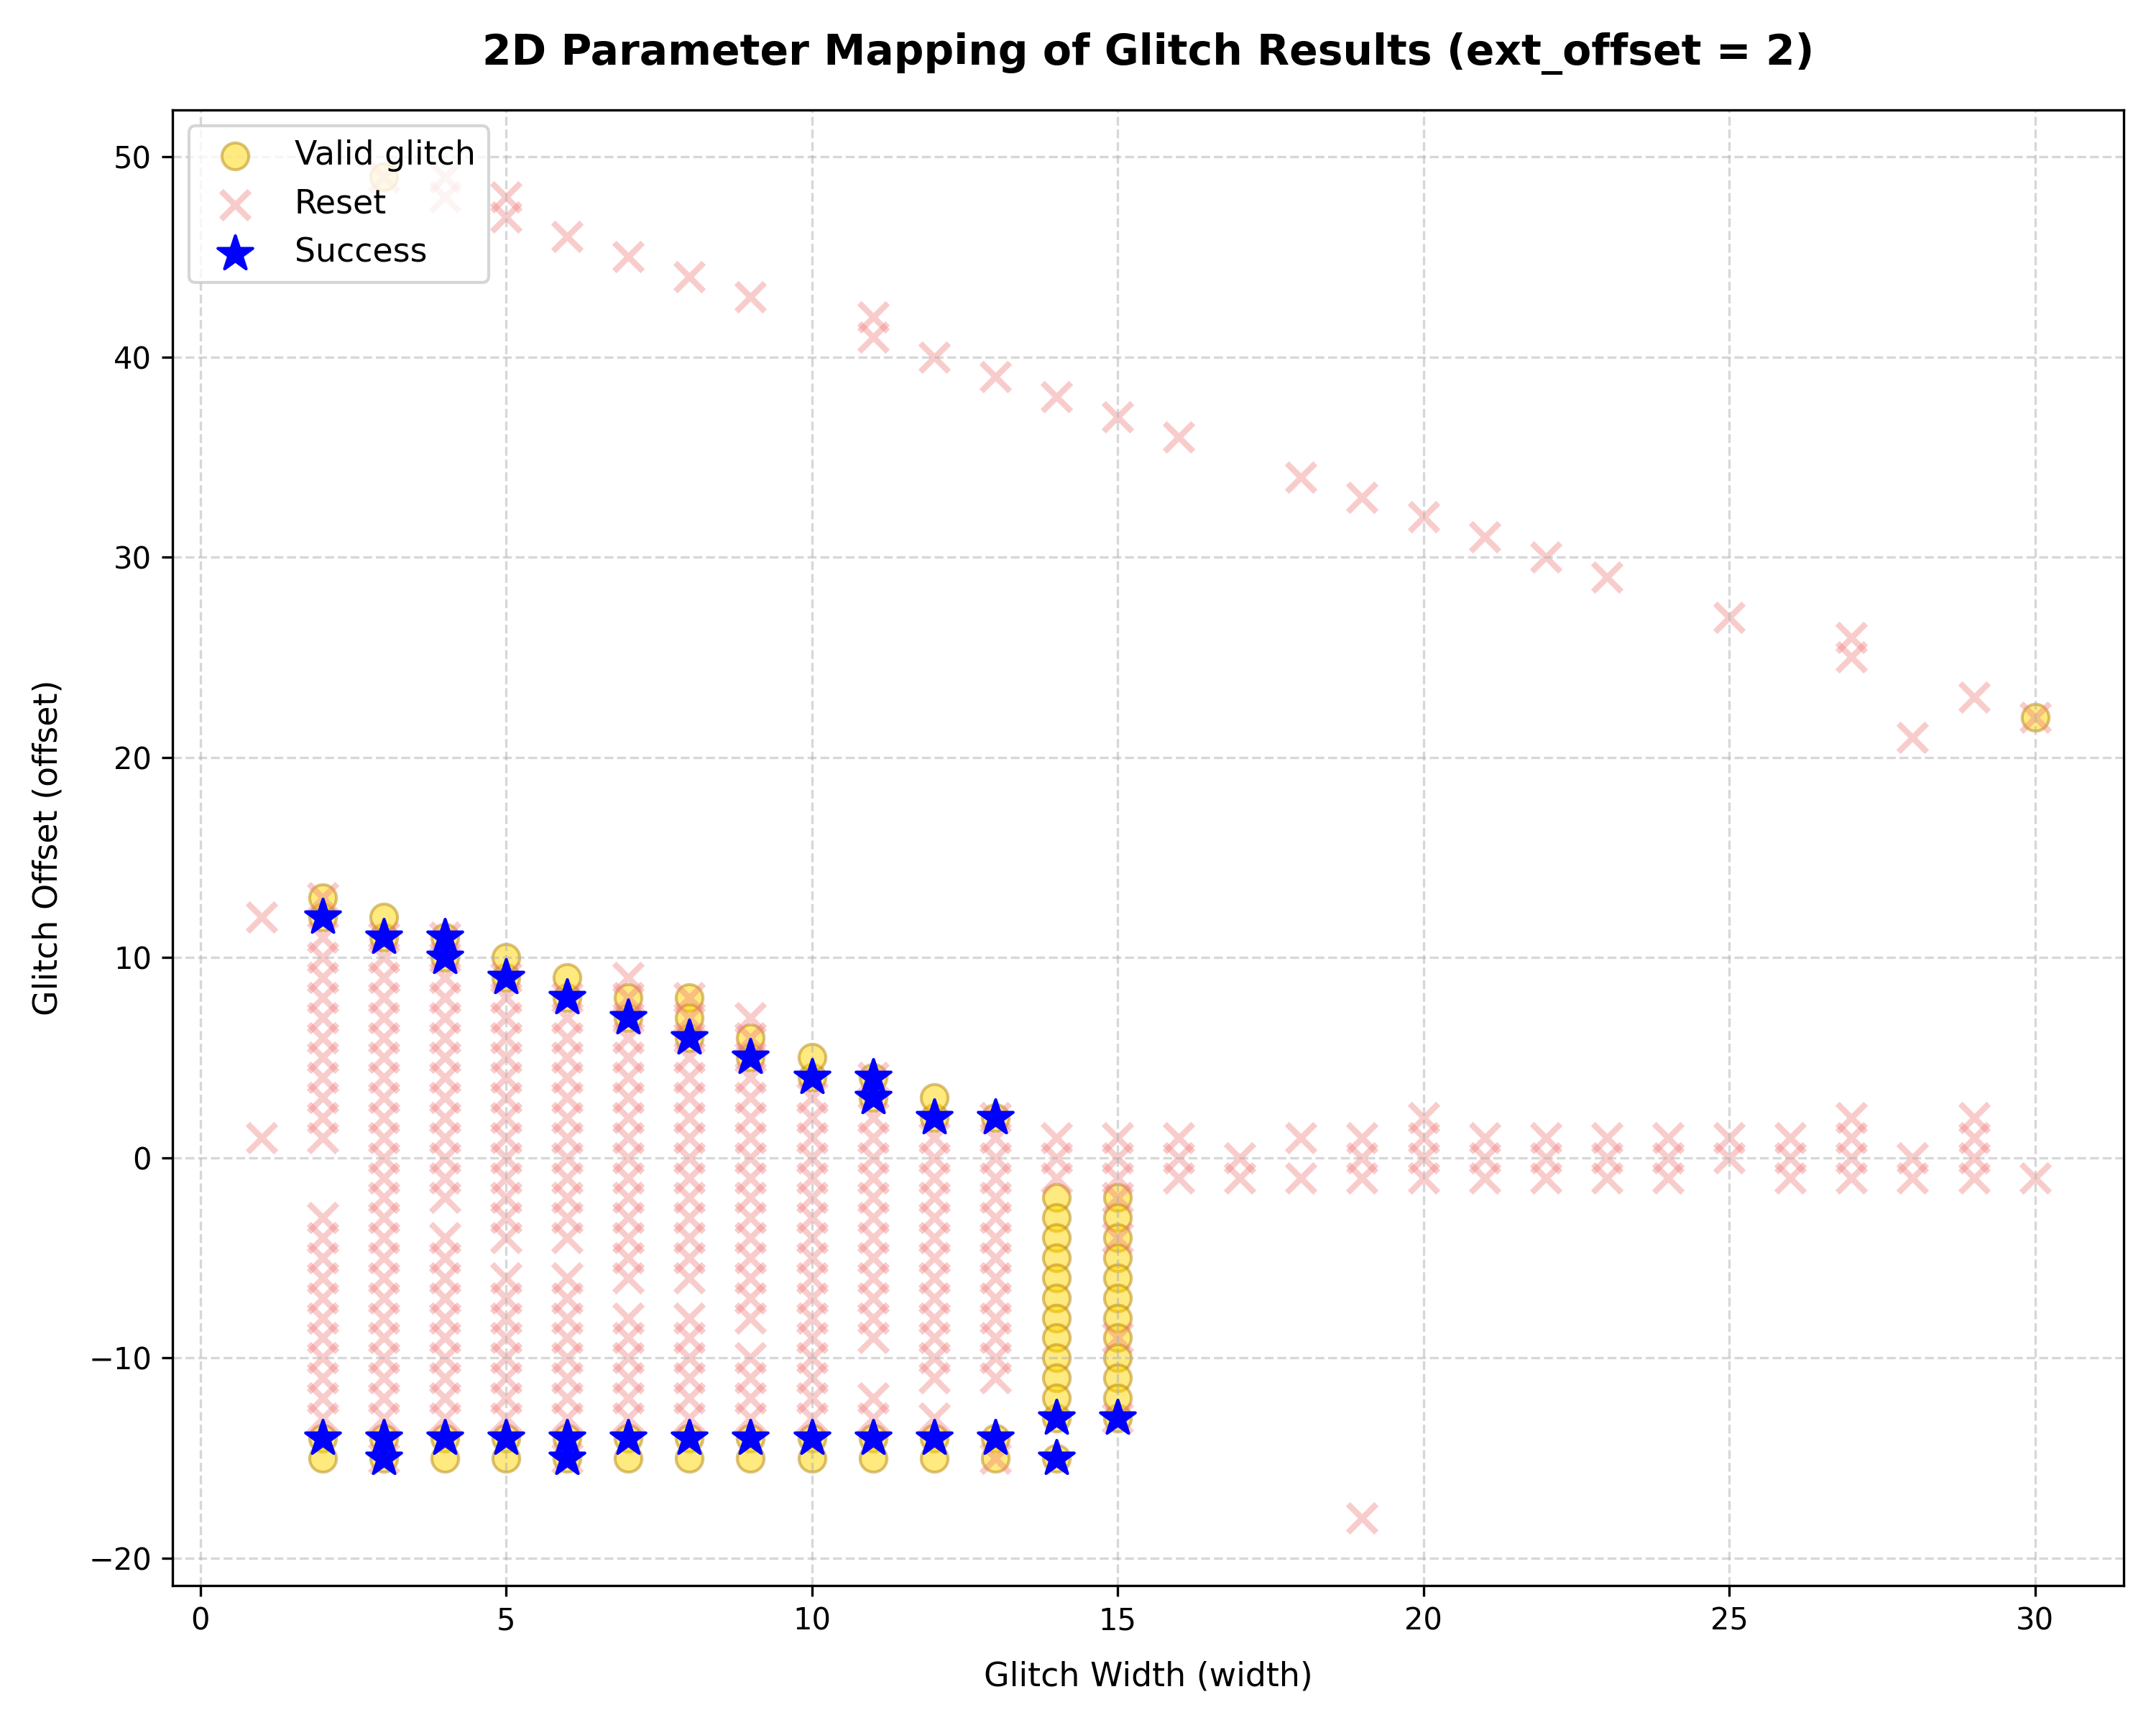
\includegraphics[width=0.58\textwidth]{content/images/glitch_2d_results_ext2.png}
    \caption{Glitch success frequency by glitch width and offset for fault model 2, with 10 tries per parameter pair.}
    \label{fig:fault2_results}
\end{figure}

We observe a distinct, bounded region of system resets delimited by successful attacks and other valid glitches. 
The paths of many of these valid glitches contain a large set of intermediate nodes which provide sufficient 
coverage to compute all of the leaf values.

\textbf{Model 3: Single hidden leaf recovery.}
In this model, we recover only a hidden leaf. 

\textit{Compilation.} Higher compiler optimization levels made it difficult to precisely target the flags. 
The  optimization flags \texttt{-O1}, \texttt{-O2}, \texttt{-O3}, and \texttt{-Os} resulted in compiled 
assembly code that omitted the explicit assignment instruction entirely, relying instead on complex control-flow 
manipulations to achieve the same logical outcome. To resolve this issue, we enforced the \texttt{-O0} optimization 
level on the targeted function, as applying \texttt{-O0} to the entire project increased 
the binary size beyond the storage capacity of the target board. 



\textit{Trigger position.} For the unoptimized version, we position the glitch high trigger right before the \texttt{index\_leaf} assignment and the low trigger right after. This results in the compiled code in listing~\ref{lst:f3asm}. 
\begin{lstlisting}[style=asmstyle, label=lst:f3asm, caption=Compiled trigger points for fault model 3.]
0800062c <stree_to_path_to_stree_glitch>:
...
 80006be:	f001 fd3f 	bl	8002140 <trigger_high> // trigger_high();
 80006c2:	2301      	movs	r3, #1             // index_leaf = 1;
 80006c4:	62bb      	str	r3, [r7, #40]	@ 0x28
 80006c6:	f001 fd43 	bl	8002150 <trigger_low>  // trigger_low();
...
\end{lstlisting}

\textit{Parameters.} The disassembled code shows that the assignement is done in two instructions which are both 1 clock cycle long. 
We set the \texttt{repeat} parameter of the glitch controller to 2. Figure~\ref{fig:fault3_results}
shows the success rate and reset for the glitch offset and width. 

\begin{figure}[htbp]
    \centering
        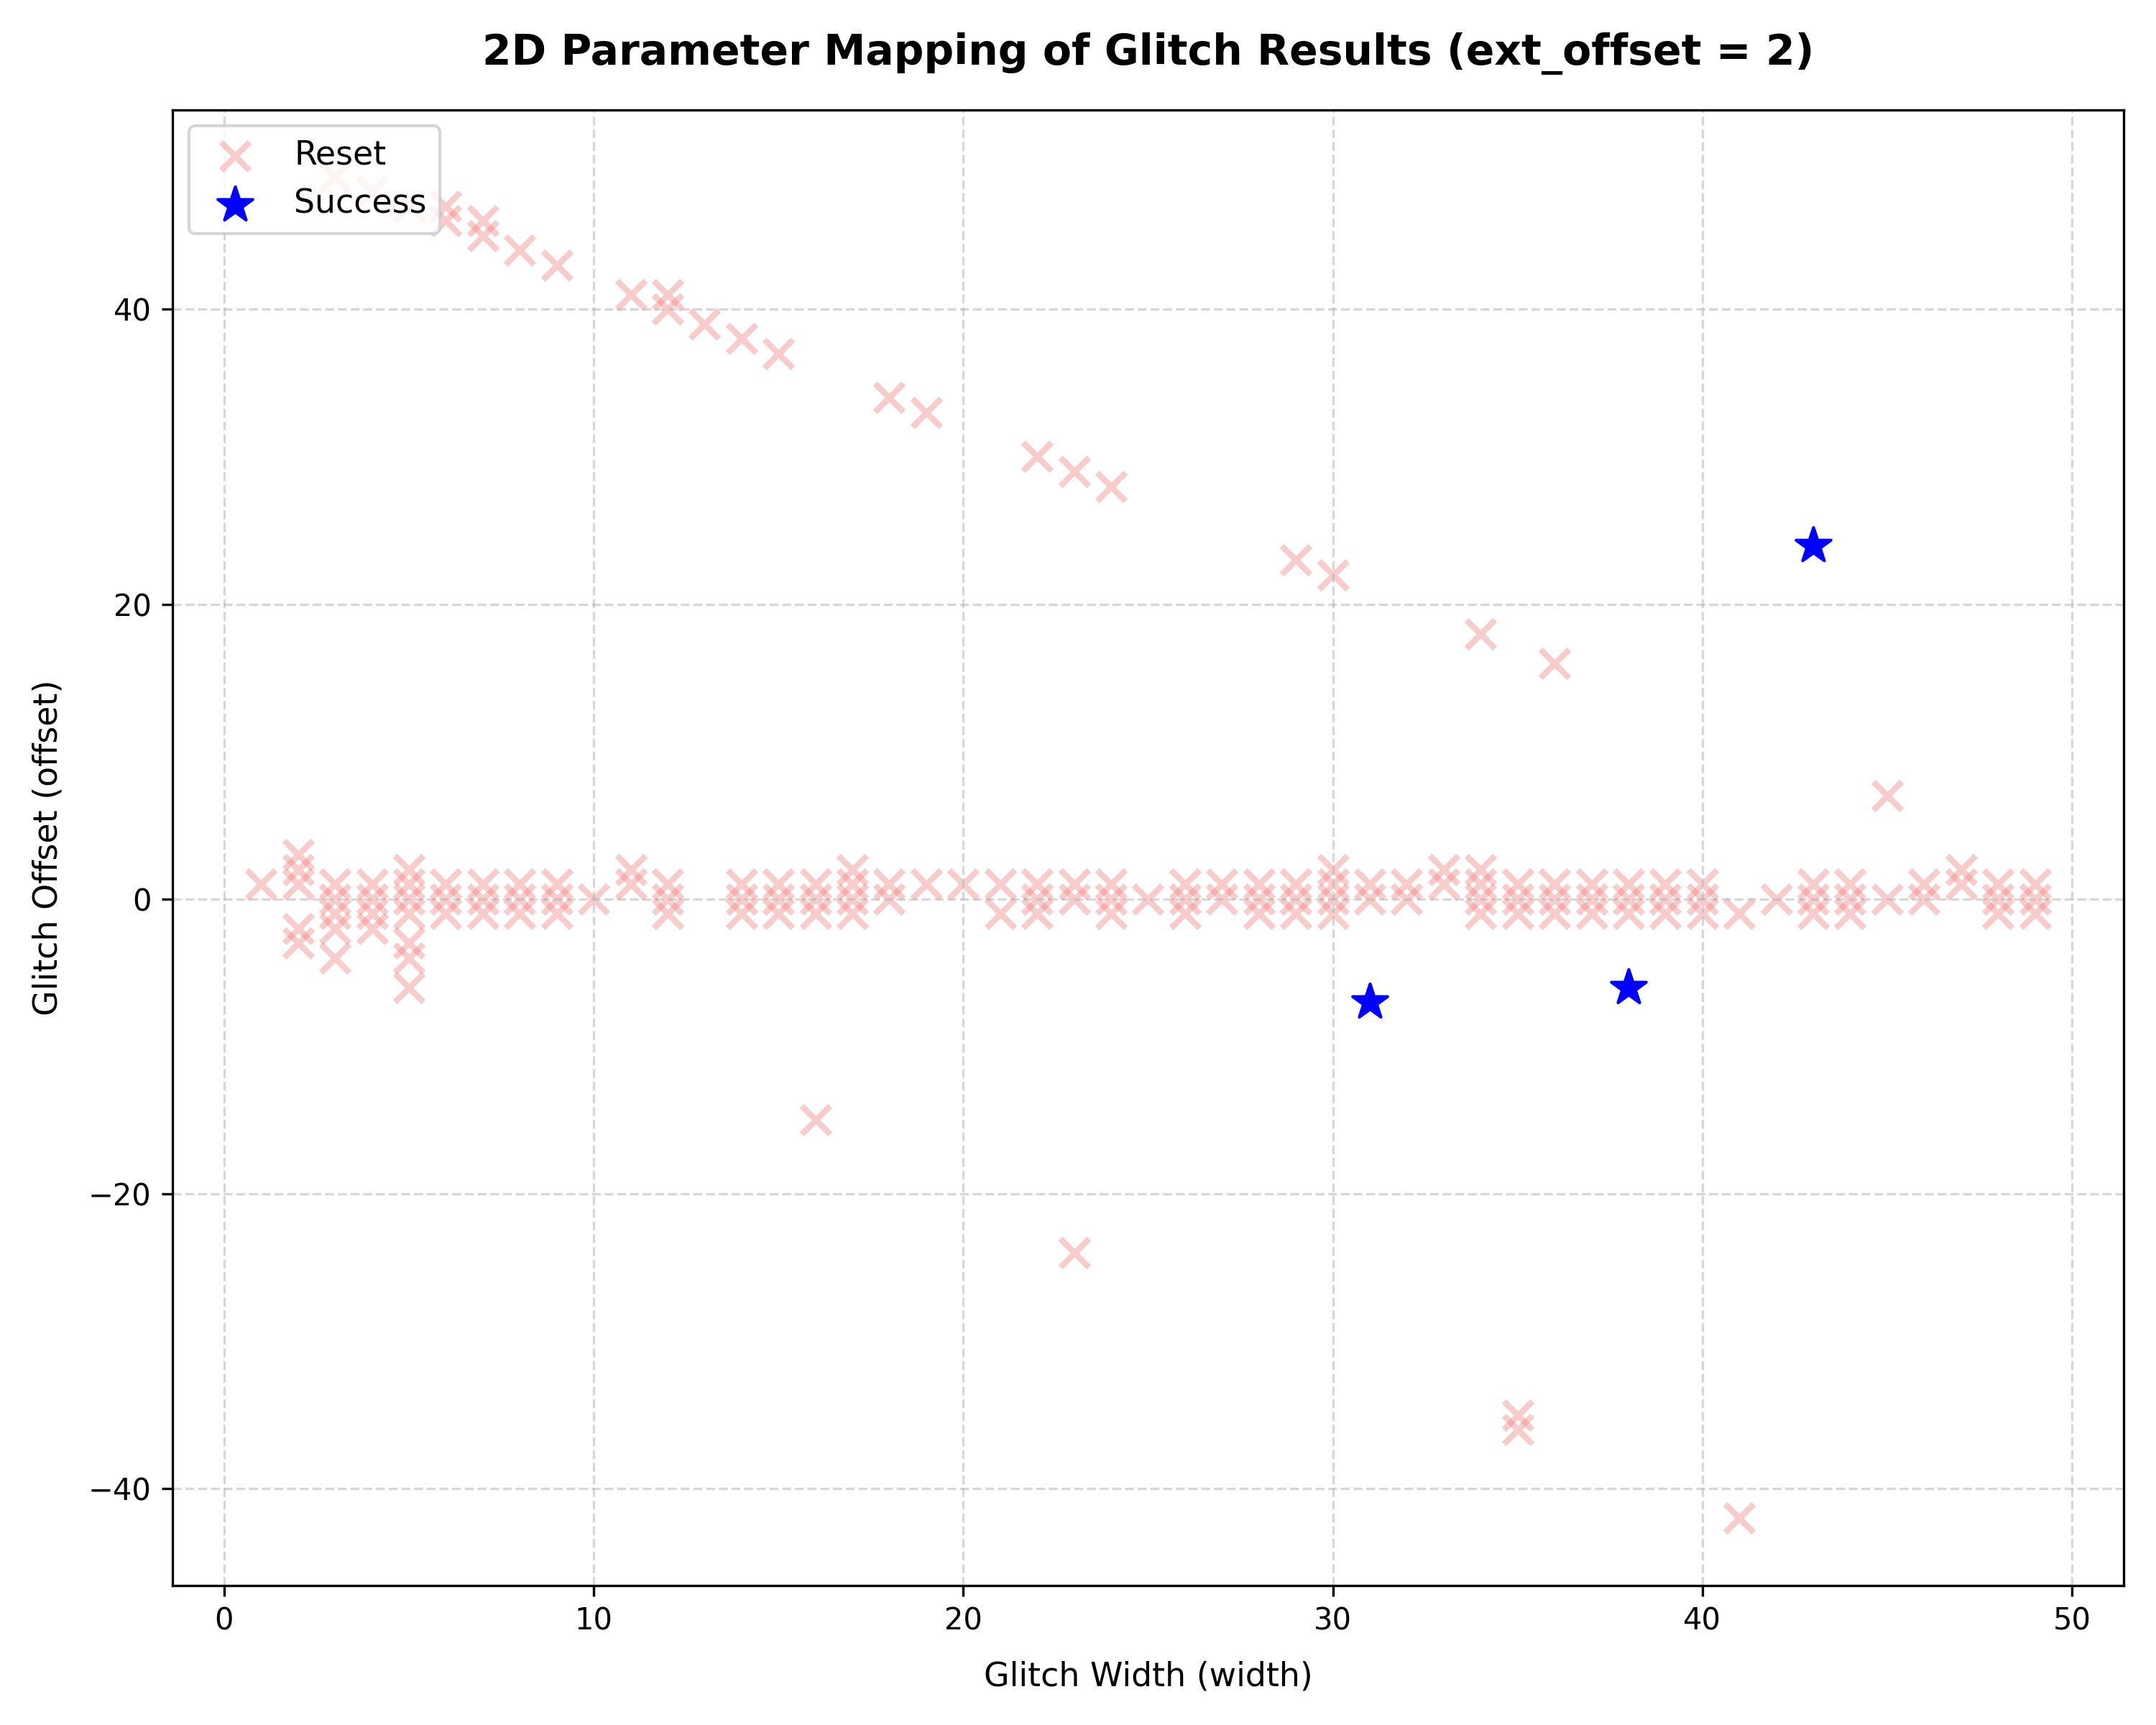
\includegraphics[width=0.58\textwidth]{content/images/glitch_2d_results_ext3.png} 
    \caption{Glitch success frequency by glitch width and offset for fault model 3, with 10 tries per parameter pair.}
    \label{fig:fault3_results}
\end{figure}

\noindent\textbf{Results.} The experiments confirm that the attack is reproducible. 
Across all parameter sweeps, attempts strictly resulted in either normal execution, a device reset, or the expected exploit. 
We observed a complete absence of other valid glitches. This is due to our single-instruction targeting. Unlike  
fault models that disrupt larger execution windows and introduce non-deterministic errors, this injection is less likely
to bleed into surrounding cycles or to trigger a control-flow collapse.

These experiments demonstrate that the root reveal fault model, which is the most efficient approach requiring 
the fewest queries for full secret key recovery, is highly reproducible. Furthermore, our results confirm the viability of two alternative fault models,
although they prove more challenging to replicate under experimental conditions. Despite their lower reproducibility rates, 
fault models 2 and 3 remain relevant for threat modeling; as detailed in Section~\ref{sec:counter}, they incur a higher computational or architectural 
cost to detect during signature generation.

\section{Countermeasures}
\label{sec:counter}
In this section we suggest a set of countermeasures that would make the signature scheme more secure against the exposed fault models.

We split the countermeasures into different categories :

\begin{itemize}
    \item Post-publication code path check : same signature size, no modification of the tree construction.
    \item Path construction algorithm change : same signature size.
    \item GGM tree-less signature : larger signature.
\end{itemize}

\subsection{Post-publication path check}

This countermeasure consists is running checks on the output of \SeedTreeToPath.

A simple size check on the path is enough to be secure against fault models 1 and 3, 
since they result in path lengths of $1$ and $\text{golden path size}+1$ respectively.
The expected path size can be computed in linear time from $\calH$. (Todo : algorithm ?).

A more thorough and correct check would be to rebuild the tree using $\PathToSeedTree$ 
on the obtained path and to compare the obtained leaves to $\calH$ and the reference tree.
This can also be done in linear time.

\begin{remark}
    In order to pass this check, it would be sufficient to induce 
    the same fault as in the $\SeedTreeToPath$ on $\PathToSeedTree$, seeing as they both 
    call the same function in the reference implementation.
\end{remark}

\subsubsection{Impact on performances}

We implement both of these checks and compare execution times of the signature step with 
or without countermeasure. The results are summarized in table~\ref{tab:counter_1_cmp}. We refer to the path size check countermeasure by $\textbf{C}_{size}$ and 
the full tree check by $\textbf{C}_{tree}$.

\begin{table}[H]
\centering
\caption{Countermeasures execution time comparison}
\label{tab:counter_1_cmp}
\setlength{\tabcolsep}{10pt}
\begin{tabular}{@{}lcc@{}}
\toprule
\textbf{Version} & \textbf{Time (min)} & \textbf{cycles} \\
 Base   &  0.001230 & 4798061  \\
$C_{size}$   &  0.001070 & 4171382  \\
$C_{tree}$   &  0.001303 & 5080762  \\

\bottomrule
\end{tabular}
\end{table}


\subsection{Path construction algorithm modification}

Though the current implementation of $\SeedTreeToPath\slash\PathToSeedTree$ is very efficient,
it allows for attack namely because it merges the flag tree construction and the path construction
steps. 

Splitting the two steps and introducting a check after both stages could limit the 
attack surface by introducing redundancy.

Todo : detail + implementation + time analysis.

\subsection{GGM-tree-less signature}

We could also consider not using GGM trees and publishing all $t-w$ seeds. 
Todo : size of the signature.

\section{Conclusion}
\label{sec:conclusion}
We presented a unified study of fault attacks against 
post-quantum signature schemes based on seed-tree compression. 
Through the GZKST abstraction, we identified a 
common seed-hiding invariant underlying schemes such as 
LESS-v2, CROSS, and MEDS, and showed that previously 
proposed attacks can be viewed as violations of this 
invariant.

Building on this framework, we derived generic key-recovery 
procedures and analyzed their query complexity. We also 
demonstrated practical clock-glitch attacks against the 
MEDS reference implementation on an ARM Cortex-M4 
microcontroller, revealing multiple fault surfaces that 
enable hidden-seed disclosure and secret-key recovery. 
Finally, we proposed and evaluated several countermeasures, 
showing that effective protections can be achieved with 
small overhead. Overall, our results highlight the 
importance of securing seed-publication mechanisms 
against implementation-level fault attacks.


\bibliographystyle{plain}
\bibliography{references}

\appendix
\section{Full Proofs}
\label{app:proofs}

Throughout this appendix, $\calT$ denotes a \GGM\ seed tree with leaf set
$\{0,\ldots,t-1\}$ and $\calF : V(\calT) \to \{0,1\}$ its flag labelling,
as produced by the $\Publish$ phase of the relevant \GZKST\ instance.
We use the convention $\calF(v) = 1$ to mean that $v$'s subtree contains at
least one hidden leaf ($i \in \calH$), and $\calF(v) = 0$ to mean that all
leaf descendants of $v$ are revealed ($i \in \calR$).

% ------------------------------------------------------------
\subsection{Proof of Proposition~\ref{prop:less-gzkst}
  (LESS-v2 is a \GZKST\ instance)}
\label{app:proof-less}
% ------------------------------------------------------------

Let $\calT$ be the LESS-v2 seed tree with $\lceil \log_2 t \rceil$ levels.
After the three-phase flag-tree construction the flag values are:
\begin{align}
  \calF(\mathrm{leaf}_i) &= \mathbf{1}[i \in \calH], \quad i \in \{0,\ldots,t-1\},
  \label{eq:leaf-flag}\\
  \calF(v) &= \calF(\ell) \vee \calF(r), \quad \text{for every internal node } v
  \text{ with children } \ell, r.
  \label{eq:or-prop}
\end{align}
Equations~\eqref{eq:leaf-flag}--\eqref{eq:or-prop} jointly imply:
\begin{equation}
  \calF(v) = 1 \iff \exists\, i \in \calH : \mathrm{leaf}_i
  \text{ is a descendant of } v.
  \label{eq:flag-char}
\end{equation}
The published path is
$\tpath = \{v : \calF(v) = 0,\; \calF(\mathrm{parent}(v)) = 1\}$
(with the convention that $\calF(\mathrm{parent}(\mathrm{root})) = 1$).

\begin{proof}[Proof of Invariant~\ref{inv:correctness} (Correctness)]
Let $i \in \calR$.  Consider the root-to-leaf path
$\pi_i = (v_0 = \mathrm{root},\, v_1,\, \ldots,\, v_d = \mathrm{leaf}_i)$.

Since $|\calH| \geq 1$ (the challenge weight satisfies $w \geq 1$), at least one
leaf has flag~$1$.  By~\eqref{eq:flag-char}, $\calF(v_0) = \calF(\mathrm{root}) = 1$.

Since $i \in \calR$, equation~\eqref{eq:leaf-flag} gives $\calF(v_d) = 0$.

Because $\calF(v_0) = 1$ and $\calF(v_d) = 0$, the path $\pi_i$ contains
at least two nodes with different flags.  Define
$k = \min\{j \in \{0,\ldots,d\} : \calF(v_j) = 0\}$.
Then $k \geq 1$ (since $\calF(v_0) = 1$), $\calF(v_k) = 0$, and
$\calF(v_{k-1}) = 1$.  Hence $v_k \in \tpath$, and $v_k$ lies on
the root-to-leaf path $\pi_i$, establishing Invariant~\ref{inv:correctness}.
\end{proof}

\begin{proof}[Proof of Invariant~\ref{inv:hiding} (ZK hiding)]
Let $i \in \calH$ and let $v$ be any proper ancestor of $\mathrm{leaf}_i$
(including the root).  Since $\mathrm{leaf}_i$ is a descendant of $v$ and
$i \in \calH$, equation~\eqref{eq:flag-char} gives $\calF(v) = 1$.
Hence no ancestor of $\mathrm{leaf}_i$ can satisfy $\calF(v) = 0$, so no
ancestor of $\mathrm{leaf}_i$ lies in $\tpath$.  Invariant~\ref{inv:hiding}
holds.
\end{proof}

\begin{proof}[Extension to incomplete trees (Remark~\ref{rem:incomplete})]
When $t$ is not a power of~$2$, the LESS-v2 tree is incomplete: some leaves
appear at depth $\lceil \log_2 t \rceil - 1$ rather than $\lceil \log_2 t \rceil$.
The index-tracking arrays $\mathsf{npl}$, $\mathsf{ll}$, $\mathsf{off}$, and
$\mathsf{lsi}$ ensure that $\LabelLeaves$ correctly identifies which nodes are
leaves and assigns flags according to~\eqref{eq:leaf-flag}, and that
$\ComputeSeeds$ performs the bottom-up OR pass~\eqref{eq:or-prop} over the
actual tree structure.

The proofs of both invariants above are purely graph-theoretic and depend only
on the properties~\eqref{eq:leaf-flag}--\eqref{eq:flag-char}, which hold
regardless of whether leaves appear at a uniform depth.  Hence both invariants
hold for any incomplete tree shape produced by the LESS-v2 expansion.
\end{proof}

% ------------------------------------------------------------
\subsection{ Proof of Proposition~\ref{prop:meds-gzkst}
  (MEDS is a \GZKST\ instance)}
\label{app:proof-meds}
% ------------------------------------------------------------

MEDS uses $\SeedTreeToPath$, which implements a top-down erasure: starting from
a fully built tree, for each $i \in \calH$ the algorithm removes the label of
$\mathrm{leaf}_i$ and propagates the removal upward, erasing every ancestor
whose entire subtree has had all labels removed.

\begin{claim}
After the erasure pass, a node $v$ retains its label if and only if
$\calF(v) = 0$ in the sense of~\eqref{eq:flag-char}, i.e., $v$'s subtree
contains no hidden leaf.
\end{claim}
\begin{proof}
A node is erased iff every leaf in its subtree has been removed, which holds
iff every leaf in its subtree is in $\calH$.  Equivalently, a node retains its
label iff its subtree contains at least one revealed leaf, i.e., $\calF(v) = 0$.
\end{proof}

The published path $\tpath$ consists of the highest surviving nodes in the tree,
serialised in depth-first order; equivalently,
$\tpath = \{v : v \text{ retains its label},\; \mathrm{parent}(v) \text{ was erased}\}$.
By the claim, this is $\{v : \calF(v) = 0,\; \calF(\mathrm{parent}(v)) = 1\}$,
which is identical to the LESS-v2 definition.

Invariants~\ref{inv:correctness} and~\ref{inv:hiding} follow by the same
argument as in Appendix~A.1.

% ------------------------------------------------------------
\subsection{Proof of Proposition~\ref{prop:cross-gzkst}
  (CROSS is a \GZKST\ instance)}
\label{app:proof-cross}
% ------------------------------------------------------------

The seed-tree component of CROSS ($\SeedTreePaths$) is structurally equivalent
to MEDS's $\SeedTreeToPath$ (see Section~\ref{sec:mapping}).  The argument of
Appendix~A.2 therefore applies directly, establishing
Invariants~\ref{inv:correctness} and~\ref{inv:hiding} for the seed-hiding part.

The additional Merkle proof over $\{\mathsf{cmt}_0[i]\}_{i \in \calH}$ is an
authenticity mechanism for the commitment digests that the verifier cannot
recompute from the revealed seeds.  It neither publishes any seed in
$\{\eseed_i : i \in \calH\}$ nor affects the seed-path computation, and is
therefore orthogonal to both invariants.

% ------------------------------------------------------------
\subsection{Proof of Proposition~\ref{prop:mpcith-gzkst}
  (MPCitH/VOLEitH family is a \GZKST\ instance)}
\label{app:proof-mpcith}
% ------------------------------------------------------------

For each epoch $e \in \{1,\ldots,\tau\}$, the tree has $N_e$ leaves with
exactly one hidden leaf at position $i^*[e]$.
$\mathsf{GetSiblingPath}$ publishes the \emph{co-path}: for each node on the
root-to-hidden-leaf path, the sibling is added to $\tpath$.

Formally, let $\pi^*_e = (u_0 = \mathrm{root},\, u_1,\, \ldots,\, u_d = \mathrm{leaf}_{i^*[e]})$
be the root-to-hidden-leaf path in epoch $e$.  The co-path for epoch $e$ is
$\tpath_e = \{ \mathrm{sibling}(u_k) : k = 1, \ldots, d \}$,
and $\tpath = \bigcup_e \tpath_e$.

\begin{proof}[Proof of Invariant~\ref{inv:correctness}]
Let $(e, i)$ with $i \neq i^*[e]$ be a revealed pair.  Let $k$ be the shallowest
level at which the path from the root to $\mathrm{leaf}_i$ and the path
$\pi^*_e$ diverge; denote the node on $\pi^*_e$ at level $k$ by $u_k$ and its
sibling by $\mathrm{sibling}(u_k)$.

Since the paths diverge at level $k$, the subtree below $\mathrm{sibling}(u_k)$
contains $\mathrm{leaf}_i$ but not $\mathrm{leaf}_{i^*[e]}$.
Since $\mathrm{sibling}(u_k) \in \tpath_e$, the verifier holds this node and
can expand its subtree downward to recover $\eseed_{(e,i)}$.
\end{proof}

\begin{proof}[Proof of Invariant~\ref{inv:hiding}]
The co-path $\tpath_e$ consists of siblings of nodes on $\pi^*_e$, never
nodes on $\pi^*_e$ itself.  In particular, no ancestor of $\mathrm{leaf}_{i^*[e]}$
is in $\tpath_e$.  Expanding any node in $\tpath_e$ downward therefore never
reaches $\mathrm{leaf}_{i^*[e]}$.

For epoch $e' \neq e$, the co-paths $\tpath_{e'}$ belong to a different
epoch's tree (or a different sub-tree of the interleaved structure), and
contain no node that is an ancestor of $\mathrm{leaf}_{i^*[e]}$.
Hence $\tpath$ contains no ancestor of any hidden leaf, establishing
Invariant~\ref{inv:hiding}.
\end{proof}

% ------------------------------------------------------------
\subsection{Proof of Proposition~\ref{prop:alg-correctness}
  (Correctness of Algorithm~\ref{alg:key-recovery})}
\label{app:proof-recovery}
% ------------------------------------------------------------

Let $m = |\calS| = s - 1$.  We model collection of secret components as a
\emph{generalised coupon-collector} problem with $m$ distinct coupons.

\paragraph{Correctness of Extract.}
For each scheme, Definition~\ref{def:extract} specifies $\Extract$ as a closed-form
algebraic procedure: matrix inversion over $\mathbb{F}_q$ (MEDS), column extraction
(LESS), a group operation (CROSS), or linear combination of shares (MPCitH).
Each procedure is deterministic and correct given the dual revelation
$(\eseed_i, \resp_i)$: the algebraic relationship between the response and the
hidden seed is an identity (not an approximation), so $\Extract$ returns exactly
$\sk' = $ the secret component indexed by $j = c_i$.

\paragraph{Termination.}
Define the \emph{progress probability} at step $q$ as
\[
  p_{\min} \;=\; 1 - \left(1 - \frac{1}{s-1}\right)^{\!\bar{w}},
\]
where $\bar{w} = w \cdot \ell / t \geq 1$ is the expected number of hidden
leaves in the subtree of $v^*$.  Since each hidden leaf's challenge index
$c_i$ is uniform in $\{1,\ldots,s-1\}$ independently of which components
have already been collected, we have
\[
  \Pr\bigl[\mathsf{new}(q) \geq 1 \;\big|\; \mathsf{Collected}\bigr]
  \;\geq\; p_{\min} \;>\; 0
  \qquad \text{for all } s \geq 2,\; \bar{w} \geq 1.
\]
Let $T_j$ be the number of effective queries to go from
$|\mathsf{Collected}| = j-1$ to $|\mathsf{Collected}| = j$.
Conditional on $|\mathsf{Collected}| = j-1$, each query succeeds with
probability at least $p_{\min}$, so $T_j$ is stochastically dominated by
a $\mathrm{Geom}(p_{\min})$ random variable, which is finite almost
surely.  Hence $Q = \sum_{j=1}^{m} T_j$ is finite almost surely, and
Algorithm~\ref{alg:key-recovery} terminates with probability~$1$.

\paragraph{Expected query count and tail bound.}
Let $R_k$ be the number of uncollected secret indices after $k$ effective
queries, and let $r = R_{k-1} > 0$.  Each of the $\bar{w}$ hidden leaves
in the subtree independently draws a uniform index from $\{1,\ldots,s-1\}$,
so the probability that \emph{none} of the $\bar{w}$ draws falls in the
remaining set of size $r$ is $\bigl((s-1-r)/(s-1)\bigr)^{\bar{w}}$.
Hence the probability of revealing at least one new index is
\begin{equation}
  p_r \;=\; 1 - \left(\frac{s-1-r}{s-1}\right)^{\!\bar{w}}
           \;=\; 1 - \left(1 - \frac{r}{s-1}\right)^{\!\bar{w}}.
  \label{eq:pr-exact}
\end{equation}
Since $r \geq 1$ and $\bigl(1 - r/(s-1)\bigr)^{\bar{w}} \leq
\bigl(1 - 1/(s-1)\bigr)^{\bar{w}}$, we have $p_r \geq p_{\min}$ for
all $r \geq 1$.

The expected total number of effective queries is
\begin{equation}
  \mathbb{E}[Q] \;=\; \sum_{r=1}^{m} \frac{1}{p_r}
  \;\leq\; \frac{m}{p_{\min}} \;=\; \frac{s-1}{p_{\min}},
  \label{eq:exp-Q}
\end{equation}
where the equality uses the standard coupon-collector identity for the
case where each query attempts $\bar{w}$ independent draws.

For the tail bound, each $T_j \leq k_0$ with probability at least
$1 - (1 - p_{\min})^{k_0}$ (geometric tail), so by a union bound over
$m = s-1$ stages,
\[
  \Pr[Q > k] \;\leq\; (s-1)\cdot(1-p_{\min})^{\lfloor k/(s-1)\rfloor}.
\]
Setting $(s-1)(1-p_{\min})^{\lfloor k/(s-1)\rfloor} \leq \delta$ and
solving gives $k \leq \bigl\lceil \tfrac{s-1}{p_{\min}} \cdot
\ln\tfrac{s-1}{\delta} \bigr\rceil$, establishing the bound in
Proposition~\ref{prop:alg-correctness}.

\paragraph{Output correctness.}
When the loop terminates, $|\mathsf{Collected}| = m$, and for each
$j \in \{1,\ldots,s-1\}$ there is exactly one entry $(j, \sk'_j) \in \mathsf{Collected}$
with $\sk'_j = A_j^{-1}$ (or the corresponding secret for each scheme).
The $\mathsf{Collect}$ step assembles these into $\widehat{\sk}$, which equals $\sk$
by correctness of $\Extract$.

% ------------------------------------------------------------
\subsection{Derivation of Proposition~\ref{prop:query-count}
  (Expected query count)}
\label{app:proof-query}
% ------------------------------------------------------------

\paragraph{Setup.}
Let $v^*$ be the faulted node with $\ell$ leaf descendants.
By the Fiat--Shamir uniformity assumption, the challenge index $c_i$ is
uniform in $\{1,\ldots,s-1\}$ independently for each
$i \in \calH \cap \mathrm{leaves}(v^*)$.
The actual number of hidden leaves in the subtree,
$L = |\calH \cap \mathrm{leaves}(v^*)|$, is a hypergeometric random variable
with mean $\bar{w} = w \cdot \ell / t$.

\paragraph{Distinct secrets per query (fixed $L = \ell_h$).}
Conditioning on $L = \ell_h$, the number of \emph{distinct} secret indices
revealed in one effective query has expectation
\begin{align}
  \mathbb{E}[\text{\#distinct} \mid L = \ell_h]
  &= (s-1)\!\left(1 - \left(1 - \frac{1}{s-1}\right)^{\!\ell_h}\right),
  \label{eq:edist-exact}
\end{align}
by linearity of expectation and symmetry of the uniform distribution.

\paragraph{Averaging over $L$ and the Jensen remark.}
Taking expectation over $L$,
\[
  \mathbb{E}[\text{\#distinct}]
  = (s-1)\!\left(1 - \mathbb{E}\!\left[\left(1-\tfrac{1}{s-1}\right)^{\!L}\right]\right).
\]
Since $f(x) = \alpha^x$ with $\alpha = 1 - 1/(s-1) \in (0,1)$ satisfies
$f''(x) = (\ln\alpha)^2 \alpha^x > 0$ (convex), Jensen's inequality gives
$\mathbb{E}[f(L)] \geq f(\mathbb{E}[L]) = \alpha^{\bar{w}}$.
Hence
\begin{equation}
  \mathbb{E}[\text{\#distinct}]
  \;\leq\; (s-1)\!\left(1 - \left(1-\frac{1}{s-1}\right)^{\!\bar{w}}\right)
  \;=:\; E_{\mathrm{dist}}.
  \label{eq:edist}
\end{equation}
That is, $E_{\mathrm{dist}}$ is an \emph{upper bound} on the true expected
number of distinct secrets per query; the exact value requires knowing the
distribution of $L$.  For a deterministic fault on a fixed node this
distinction vanishes ($L$ is determined by the challenge), so
$E_{\mathrm{dist}}$ is exact when conditioned on a specific query.

\paragraph{Total queries.}
From equation~\eqref{eq:pr-exact} in Appendix~A.5,
$p_r = 1 - \bigl((s-1-r)/(s-1)\bigr)^{\bar{w}}$,
and the coupon-collector identity gives
\[
  \mathbb{E}[Q] = \sum_{r=1}^{m} \frac{1}{p_r} \leq \frac{m}{p_{\min}}
  = \frac{s-1}{p_{\min}},
\]
since $p_r \geq p_{\min}$ for all $r \geq 1$.  Note that
$p_{\min} = E_{\mathrm{dist}}/(s-1)$, so this bound equals
$(s-1)^2/E_{\mathrm{dist}}$, which for $p_{\min} \approx 1$ (large~$w$)
gives $\mathbb{E}[Q] \lesssim s-1$.


\end{document}
